
% University Assignment Title Page
% LaTeX Template
% Version 1.0 (27/12/12)
%
% This template has been downloaded from:
% http://www.LaTeXTemplates.com
%
% Original author:
% WikiBooks (http://en.wikibooks.org/wiki/LaTeX/Title_Creation)
%
% License:
% CC BY-NC-SA 3.0 (http://creativecommons.org/licenses/by-nc-sa/3.0/)
%
% Instructions for using this template:
% This title page is capable of being compiled as is. This is not useful for
% including it in another document. To do this, you have two options:
%
% 1) Copy/paste everything between \begin{document} and \end{document}
% starting at \begin{titlepage} and paste this into another LaTeX file where you
% want your title page.
% OR
% 2) Remove everything outside the \begin{titlepage} and \end{titlepage} and
% move this file to the same directory as the LaTeX file you wish to add it to.
% Then add \input{./title_page_1.tex} to your LaTeX file where you want your
% title page.
%
%%%%%%%%%%%%%%%%%%%%%%%%%%%%%%%%%%%%%%%%%


%----------------------------------------------------------------------------------------
%	PACKAGES AND OTHER DOCUMENT CONFIGURATIONS
%----------------------------------------------------------------------------------------

\documentclass{article}
\usepackage{textcomp}
\usepackage{afterpage}
\usepackage{cite}
\usepackage{rotating}
\usepackage{booktabs}
\usepackage{float}
\usepackage{amsmath}
\usepackage{hyperref}
\usepackage{cleveref}
\usepackage{mathtools}
\usepackage[titletoc]{appendix}
\usepackage{multicol}
\usepackage[]{graphicx}
\usepackage[export]{adjustbox}
\usepackage{multicol}
\usepackage{subcaption}
\usepackage{caption}
\usepackage[font=small,labelfont=bf]{caption}
\usepackage{enumitem}
\usepackage{pdfpages}
%step 1, step 2, etc.
\newlist{steps}{enumerate}{1}
\setlist[steps, 1]{label = Step \arabic*:}
%end
\usepackage{listings}
\usepackage{url}
\usepackage{tabto}
\usepackage{hyperref}
\usepackage{babel}
\usepackage[top=1in,bottom=1in,left=1.25in,right=1.25in]{geometry}
\setlength{\parindent}{2em}

\usepackage{array,multirow,graphicx}

\usepackage{color} %red, green, blue, yellow, cyan, magenta, black, white
\definecolor{mygreen}{RGB}{28,172,0} % color values Red, Green, Blue
\definecolor{mylilas}{RGB}{170,55,241}

\usepackage{datetime}
\newdateformat{monthyeardate}{%
  \monthname[\THEMONTH], \THEYEAR}

\usepackage{caption}
%\captionsetup[table]{skip=5pt}

\usepackage{gensymb}
\usepackage{fancyhdr}
\fancyhf{}
\fancyhead[C]{\thepage}
\pagestyle{fancy}
\renewcommand{\headrulewidth}{0pt}
\usepackage{wrapfig}
\usepackage{comment}

\makeatletter
\renewcommand{\numberline}[1]{#1~}
\makeatother

% redefine the plain pagestyle
\fancypagestyle{plain}{%
\fancyhf{} % clear all header and footer fields
\fancyhead[C]{\thepage} % except the center
}
\setcounter{tocdepth}{2}


\usepackage{mwe}


\begin{document}

%Title

\pagenumbering{roman}
\begin{titlepage}

\newcommand{\HRule}{\rule{\linewidth}{0.5mm}} % Defines a new command for the horizontal lines, change thickness here

\center


{ \huge \bfseries Title of the document}\\[1cm] % Title of your document
 





\vfill
\begin{minipage}{0.4\textwidth}
    \begin{flushleft}
        TU Delft, Faculty of Applied Sciences,\\
        BSc program Applied Physics
    \end{flushleft}
\end{minipage}
~
\begin{minipage}{0.4\textwidth}
    \begin{flushright}
        Delft, April 3rd 2020\\
        van Loon, Reinaart\\
        Sangers, Jeroen
    \end{flushright}
\end{minipage}\\[1.5cm]


\end{titlepage}

\addcontentsline{toc}{section}{Abstract}
\section*{Abstract}
In this report the reader will be informed about the experiments performed for the Microscopy research project.\\
For the experiments a Leice DM EP polarising microscope in combination with a CCD camera was used to determine the magnification of certain object lenses, the width of a human hair and optical fibre, the resolving power for multiple different numerical aperatures, the cross section of elliptical starch particles and the birefringence of an unknown crystal. Finally, an image of a biological sample will be improved by using different python algorithms.\\
The magnification and resolving power of the object lenses, the width of a human hair and optical fibre and the cross section of starch particles were found by making images using the CCD camera and counting pixels. This yielded the following results: For the magnification we found pixel lengths equal to $1.5\cdot10^{-6}$, $6.4\cdot10^{-7}$ and $1.6\cdot10^{-7}$ for the $4\times$, $10\times$ and $40\times$ objectives respectively. For the width of a human hair and optical fibre; diameters of $d_{hair}=6.6\pm0.1\cdot10^{-5}$ and $d_{fiber} = 1.26\pm0.01\cdot10^{-4}$ meters were found. The mean cross section of elliptical starch particles was found to be $A_{starch}=1.9\cdot10^{-10}$ $m^2$ with a standard deviation $\sigma = 8 \cdot10^{-11}$ $m^2$. The size measurements yielded results that matched literature. However, the measurements on the starch particles turned out to be inadequate given the shape and number of unresolvable particles.\\
Determining the birefringence of the crystal was done by placing the crystal between to polarising filters and then measuring the difference in height between two colour planes, using this thickness and the colour of the plane, a birefringence number of $\delta n = 5.3\pm0.2\cdot10^{-2}$ was found. Therefore, the crystal could either be astrophylite, silk or piemontite. Given that there is an unidentified measurement error, the validity of the outcome is debatable.\\
Improving the image using the sigmoid function and a contrast enhancing rank filter works well, significantly improving the contrast of the image. A bilateral mean filter proves to be of use when removing noise. It does however, remove some of the details. A morphological contrast enhancement filter can be useful for size measurements or line detection. Combination of the different rank filters also seems to be useful to either reveal much detail or to remove noise, compensated by gain of contrast.
\newpage

% Table of contents
\thispagestyle{empty}
\addcontentsline{toc}{section}{Table of contents}
\tableofcontents
\clearpage

% Content

\newpage
\pagenumbering{arabic}
\section{Introduction}
Microscopes are used extensively in natural sciences. They enable us to image small objects and structures which cannot be resolved by the human eye. The use of microscopes, could for example, aid in studies of biological cells, molecular structures or object classification. To correctly conduct such microscopy studies, it is vital to know what the possibilities and limits are using a the particular microscope are in combination with image improvement techniques.\\
This experiment will focus on a Leica DM EP polarising microscope in combination with a colour CCD and to what extent this set-up can be used to measure the size of small objects and find the birefringence of an unknown crystal. Furthermore, the possibilities of digital image improvement will be investigated.\\
After calibrating the pixels and finding the resolving power with the aid of a microscopic ruler and resolution target, images are made of a human hair, an optical fibre, starch particles, an unknown birefringent crystal and a fungus sample.\\
To find the size of the human hair, fibre and particles, computer techniques will be used. The birefringence of the crystal will be determined by focussing on the differently coloured planes of the crystal. Using this to find the thickness of each colour plane and its colour, the birefringence can be calculated. Finally some python algorithms are implemented on the image of the fungus to investigate improvements on contrast and noise reduction.\\
In section 2 the theory regarding the experiment will be described, followed by the experimental method in section 3. The results and discussion can be found in section 4. Lastly the conclusions in section 5.









\begin{comment}
    TheInleiding ( Introduction) describes:   -The  research  question.  (Be  as  precise  as  possible.  Not:  “We  investigate  on  which  parameters  the  bubble  behaviour  depends”,  but  “we  study  the  relationship  between  the  path  of  bubbles  at  a  microfluidic T-junction, and the velocity and length of those bubbles).\\-The relevance of the research question (for science and/or technology).\\-The state-of-art: what is already know? (including references to prior literature).\\-A brief description of the research method/approach.\\-A brief description of the structure/contents of the rest of the report.\\The  introduction  should  be  self-contained,  without  reference  to  the  manual  or  to  the  remainder  of  the  report, and should be understandable to readers who know nothing about the research.
\end{comment}
\newpage
\section{Theory}
In  theTheorie  (Theory)  chapter,  you  describe  all  (and  only!)  the  theory needed  to  understand  and  interpret the experiments  in  the  remainder  of  the  report.    Explain  to  the  reader  why  a  piece  of  theory  is  relevant  for  your  research.  Equations  should  be  numbered.  If  an  equation  cannot  be  assumed  to  be  generally known by the readers (see General Hint 2 for the level of the audience), you should provide a reference to an accessible textbook or article (so not to the RP manual, lecture notes, Wikipedia etc.). In general, try to avoid referring to websites, online data or Wikipedia.
\newpage
\section{Experimental method}

This experiment consists of four parts. First the calibration of the microscope. Secondly size measurements on respectively a human hair, an optical glass fibre and starch particles. Thirdly determining the birefringence of an unknown crystal and finally the computerized improvement of an image of a biological fungus sample. The different experimental methods will be treated separately. 

The microscope that is used in all experiments is a Leica DM EP microscope. Its manual can be found in appendix \ref{appendix_manual}. This microscope is used in combination with $4\times$, $10\times$, $40\times$ Hi Plan POL objectives with respectfully a 0.10, 0.22 and 0.65 numerical aperture. A color ccd camera in combination with NI Vision Assistant software is used to acquire digital images.

\subsection{Calibration}
A microscopic ruler is used to measure the length that corresponds to one pixel in an image. This is achieved by focussing on a 1 mm, 100 division ruler and measuring the distance, $d$, between two focussed, distant division lines and comparing the number of pixels, $n$, to the physical length. The NI software is used to find the exact location of these two lines and subsequently find the perpendicular projection. This procedure is repeated for all three objectives.

With the aid of a 1951 USAF resolution target, the resolving power of each objective can be found. First taking a focussed grayscale image  on the target and then taking a perpendicular intensity profile for each well defined three-bar structure. The visibility can subsequently be calculated with equation \ref{eq_visibility}, the values for the maximum and minimum pixel value for each three-bar structure and the corresponding spatial frequency. This is repeated for all three objectives.

\subsection{Microscopic size measurements}

All microscopic size measurements are made by measuring pixels and comparing this to the corresponding pixel length. This is done for images with the $40\times$ objective since this gives the smallest error.

\subsubsection{Human hair and optical glass fibre}

Measuring the thickness of the human hair and optical glass fibre is done with the aid of the NI Vision software. First finding the two straight lines of the outer edges and subsequently measuring the perpendicular distance between the two (see Figure \ref{fig_pixellength_example}). 

\subsubsection{Starch particles}

In order to measure the size of individual starch particles, a small amount of starch is mixed with oil. Images are taken at different locations in the mixture. For ellipse-shaped particles that are focussed in the image, an ellipse can manually be fitted.

For this experiment it was chosen to find the ellipse size for 30 particles.


\subsection{Birefringence}

In order to find the birefringence, $\delta n$, of the unknown crystal, it is placed in the microscope with the polariser crossed with respect to the analyser. The crystal is then turned until bright colours can be seen. Now the path difference, $\delta l$, is measured as a function of the thickness, $D$, of the crystal. $D$ can be found by viewing a border between adjacent colour planes and subsequently noting the focussing position, $f$, of each colour plane. Taking the difference between two values of $f$ will give the difference in thickness, $d$, between two colour planes. The bottom of the sample (black) is also to be taken into account with the same procedure as described above. 

For this experiment it was chosen to find $D$ and $\delta l$ for 5 colour planes. The focussing process was repeated 4 to 5 times for every border that was studied.








\begin{comment}
The Experimentele opstelling or Experimentele  methode (Experimental  set  up  or  Experimental method) chapter describes the experimental setup and the experimental methods used in sufficient detail such that a reader can judge the soundness and, in principle, may verify the conclusions of your research. Also,  this  chapter  should  be  informative  for  a  reader  who  wants  to  perform  similar  research.  Preferably  use clear sketches of the setup, rather than photographs. In this chapter you also describe the accuracywith which direct observables have been measured, and the accuracy of the important deduced quantities. Detailed accuracy calculations should be put in an Appendix
\end{comment}

\newpage
\section{Results and discussion}
In theResultaten en discussie (Results and discussion) chapter, you present your results, generally in the form of graphs, and you discuss them. A single small table (m aximum ~10 rows x ~5 columns) is acceptable, but large tables should be in an appendix. In deviation from what many students believe, it is not desirable to separate the presentation and the discussion of results from each other. In professional literature, this is most often done together.\\ •You should introduce each graph:\\ -Why has this graph been included in the report. (What do we want to learn from this graph?).\\-Why   have   you   plotted   this   Y-axis   variable   as   a   function   of   this   X-axis   variable   (which   theoretical/expected relationship is tested/demonstrated in this this graph? \\•Then you tell the reader what (according to you) he/she should see in the graph, limiting yourself toconclusions  that  are  relatively  indisputable.  The  more  speculative  conclusions  should  be  in the  next  chapter.
\newpage
\subsection{Resolving power}
The photos of the resolution target (of which figure \ref{fig:resolution_target} is a example) were shot with the NI Vision software present on the computer we used, using this software we were able to directly create datasets for the linetraces over several groups. This meant that we had no extra artifacts from compression of the photo files. The data was exported as a comma-seperated data file. After trimming the data we used a simple python program to parse the data. The resulting figures were easily readable. One of these figures is shown below in figure \ref{fig:linetrace}\\
\vspace{-5mm}
\begin{figure}[h!]
    \centering
    \begin{minipage}{.5\textwidth}
      \centering
      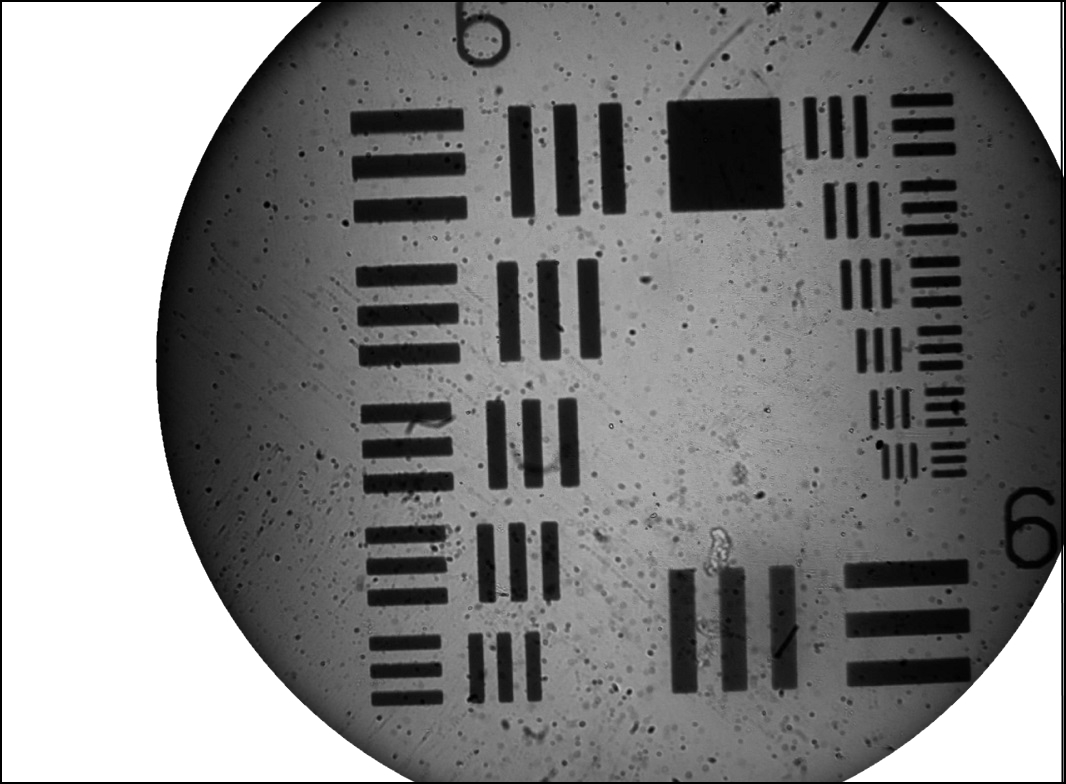
\includegraphics[width=0.7\textwidth,keepaspectratio]{afbeeldingen/process_visibility/m3_bw.jpg}
      \caption{Black and white photo.}
      \label{fig:resolution_target}
    \end{minipage}%
    \begin{minipage}{.5\textwidth}
      \centering
      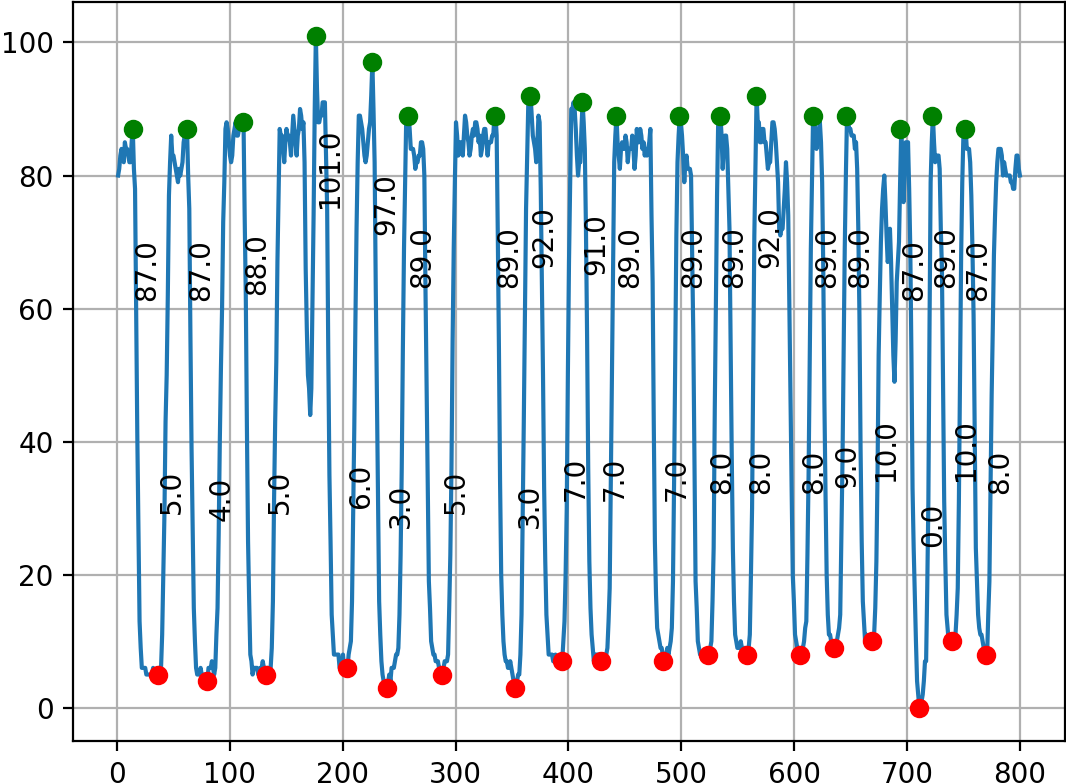
\includegraphics[width=0.7\textwidth,keepaspectratio]{afbeeldingen/process_visibility/m3_rpg_7.png}
      \caption{Linetrace of seventh group.}
      \label{fig:linetrace}
    \end{minipage}
\end{figure}

The high an low values of the line trace were manually read of the photos and entered into a python script capable of calculating the visibility values for each numerical aperature and spatial frequency. The result of which can be seen in figure \ref{fig:visibilities}.\\

\begin{wrapfigure}{l}{0.55\textwidth}
    \centering
    \vspace{-3mm}
    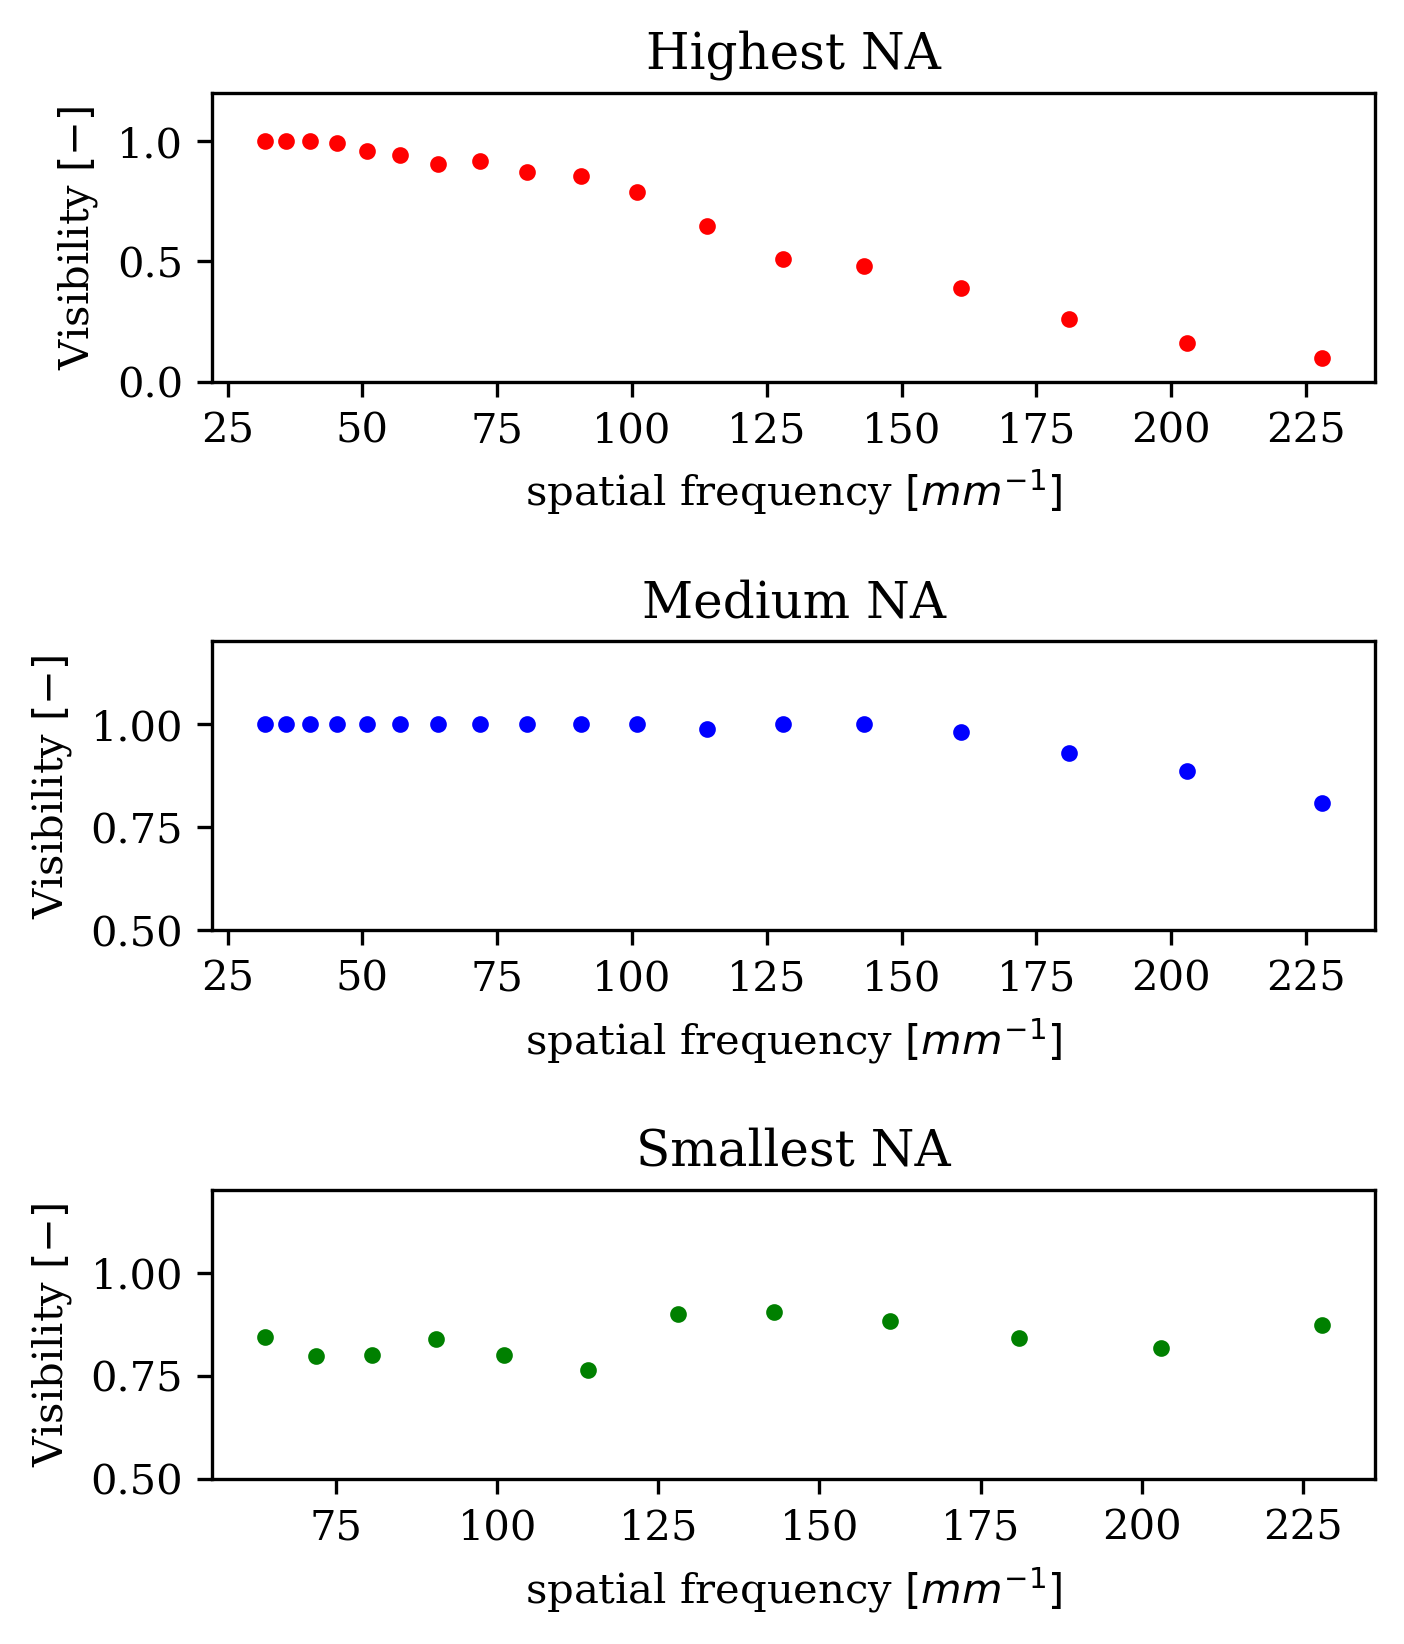
\includegraphics[width=0.55\textwidth,keepaspectratio]{afbeeldingen/visibilities.png}
    \caption{Plots of the visibilities per numerical aperature.}
    \label{fig:visibilities}
    \vspace{0mm}
\end{wrapfigure}

\vspace{-7mm}
The data is plotted in such a way that the highest subplot has the highest numerical aperature and the lowest subplot has the lowest numerical aperature. Each subplot has the dimensionless visibility number plotted on the vertical axis and the spatial frequency plotted on the horizontal axis. We chose this layout since we expect the visibility to decrease when the lines get closer together and the spatial frequency thusly increases. Note that only the verticle visibility axis of the highest subplot starts with a visibility of zero.\\
What we see is not surprising when we also take into account the photos in the appendix. As can be seen on these photos the smallest numerical aperature lense has the highest magnification, therefore all three traced groups are clearly resolvable. Thus the visibility won't drop as much as the highest aperature lense when the spatial frequency increases.\\
Something noticable however is that the smallest numerical aperature plot starts of with the lowest visibility value. This has to do with the fact that this smaller aperature aslo catches less light, the brightest spot in its photo is evidently less bright than that of the other two aperatures. This can be seen when taking a look at either the lintraces or the photos in the appendix.
\newpage
\section{Conclusions}
The experimental set-up made the pixel calibration trivial, the NI Vision software greatly increased the productivity of the work flow. Pictures of the microscopic ruler were easily translated to magnification measurement by the use of edge detection and automatic pixel counting software.\\
NI Vision also proved to be helpful with determining the resolving power of the multiple magnification objectives by being able to export a line trace of the pixel intensity, this line trace was easily readable and could thus be plotted in a graph to find the highest and lowest intensity pixel value for each given bar structure from the USAF target. These high and low values allowed for the calculation of our Visibility. The results were as expected apart from the fact that the highest magnification objective had a lower visibility starting point, this however was explained by the fact that this object had an overall lower intensity image because its low numerical aperture meant it caught less light.\\
The images of the human hair and optical fibre were made by focussing them with the smallest magnification first and then, when they were in frame and sharp, switching to a higher magnification set-up. For the starch particles the same method was used. Both yielded results that matched current literature.\\
Determining the birefringence of the crystal proved quite a bit more difficult than the previous tasks. We found that the knob to adjust the height of the sample had a bit of play, meaning that sizing the layers was hard and thus our results for the layer thickness were unreliable at best. This means that our birefringence value has quite a lot of error.
\\
Waardes er nog in, resultaten python moeten er nog in.\\
\\






\begin{comment}

In theConclusies (Conclusions) chapter\\-You give a clear and concise answer to the research question that was formulated in the Intrduction\\-You discuss  to  what  extent,  and  why,  your  findings  do  (not)  agree  with  theory/expectations/earlier  work,   you   discuss   more   speculative   conclusions,   ad   you   may   do   suggestions   for   further   (improved/extended) research.The  Conclusions  should  be  self-contained  and  understandable  for  readers  that  have  only  read  the  introduction  (and  have  not  read the  rest  of  your    report,  do  not  know  the  literature,  do  not  know  the  experimental  setup  and  have  not  read  the  RP  manual).   In  the  Conclusions  chapter,  you  may  not  make  references to graps, tables, equations etc. in the remainder of the report.

\end{comment}
\newpage
\input{literatuurlijst.tex}

%\input{tradeoff}

%Bibliography
\newpage
\addcontentsline{toc}{section}{List of references}
\bibliographystyle{ieeetr}
\bibliography{report}
\newpage
\pagenumbering{roman}

\begin{appendix}
\addcontentsline{toc}{section}{Appendices}
\renewcommand{\thesubsection}{Appendix \Alph{subsection}}


\subsection{Leica DM EP manual}
\label{appendix_manual}

\begin{figure}[h!]
	\centering
	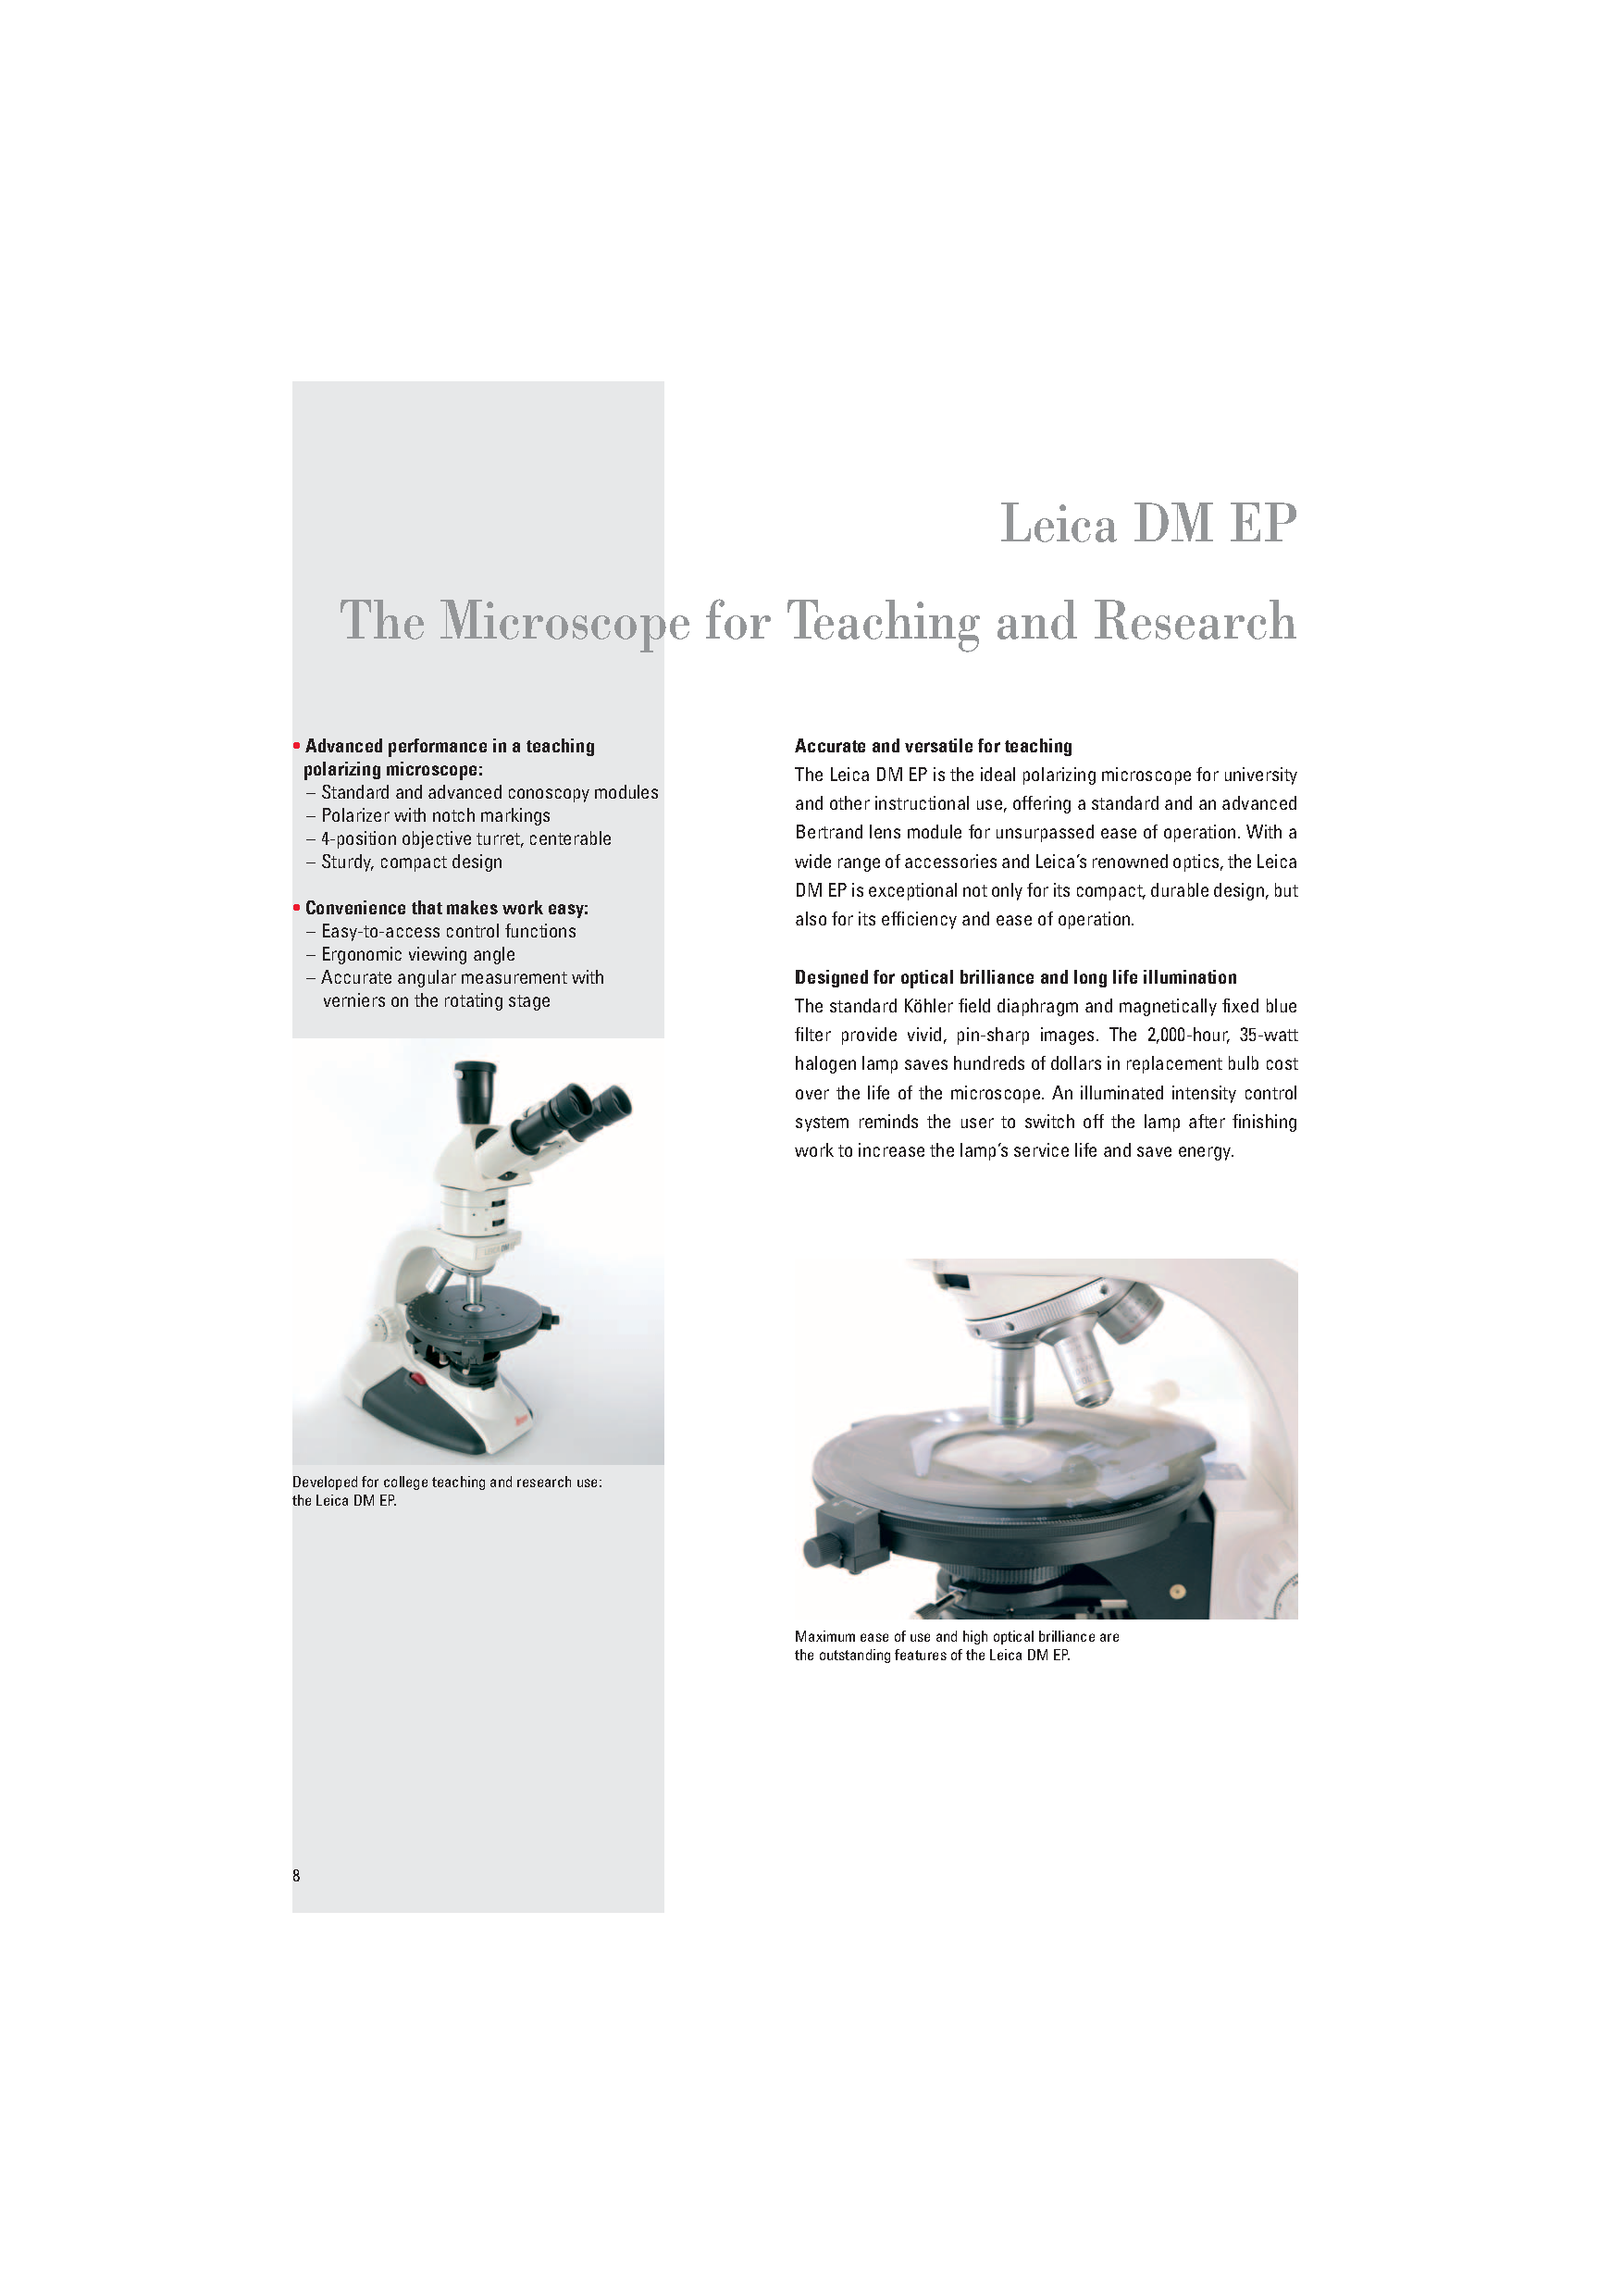
\includegraphics[width=0.9\textwidth]{afbeeldingen/manual_cut_1.pdf}
\end{figure}
\newpage	
\begin{figure}[h!]
	\centering
	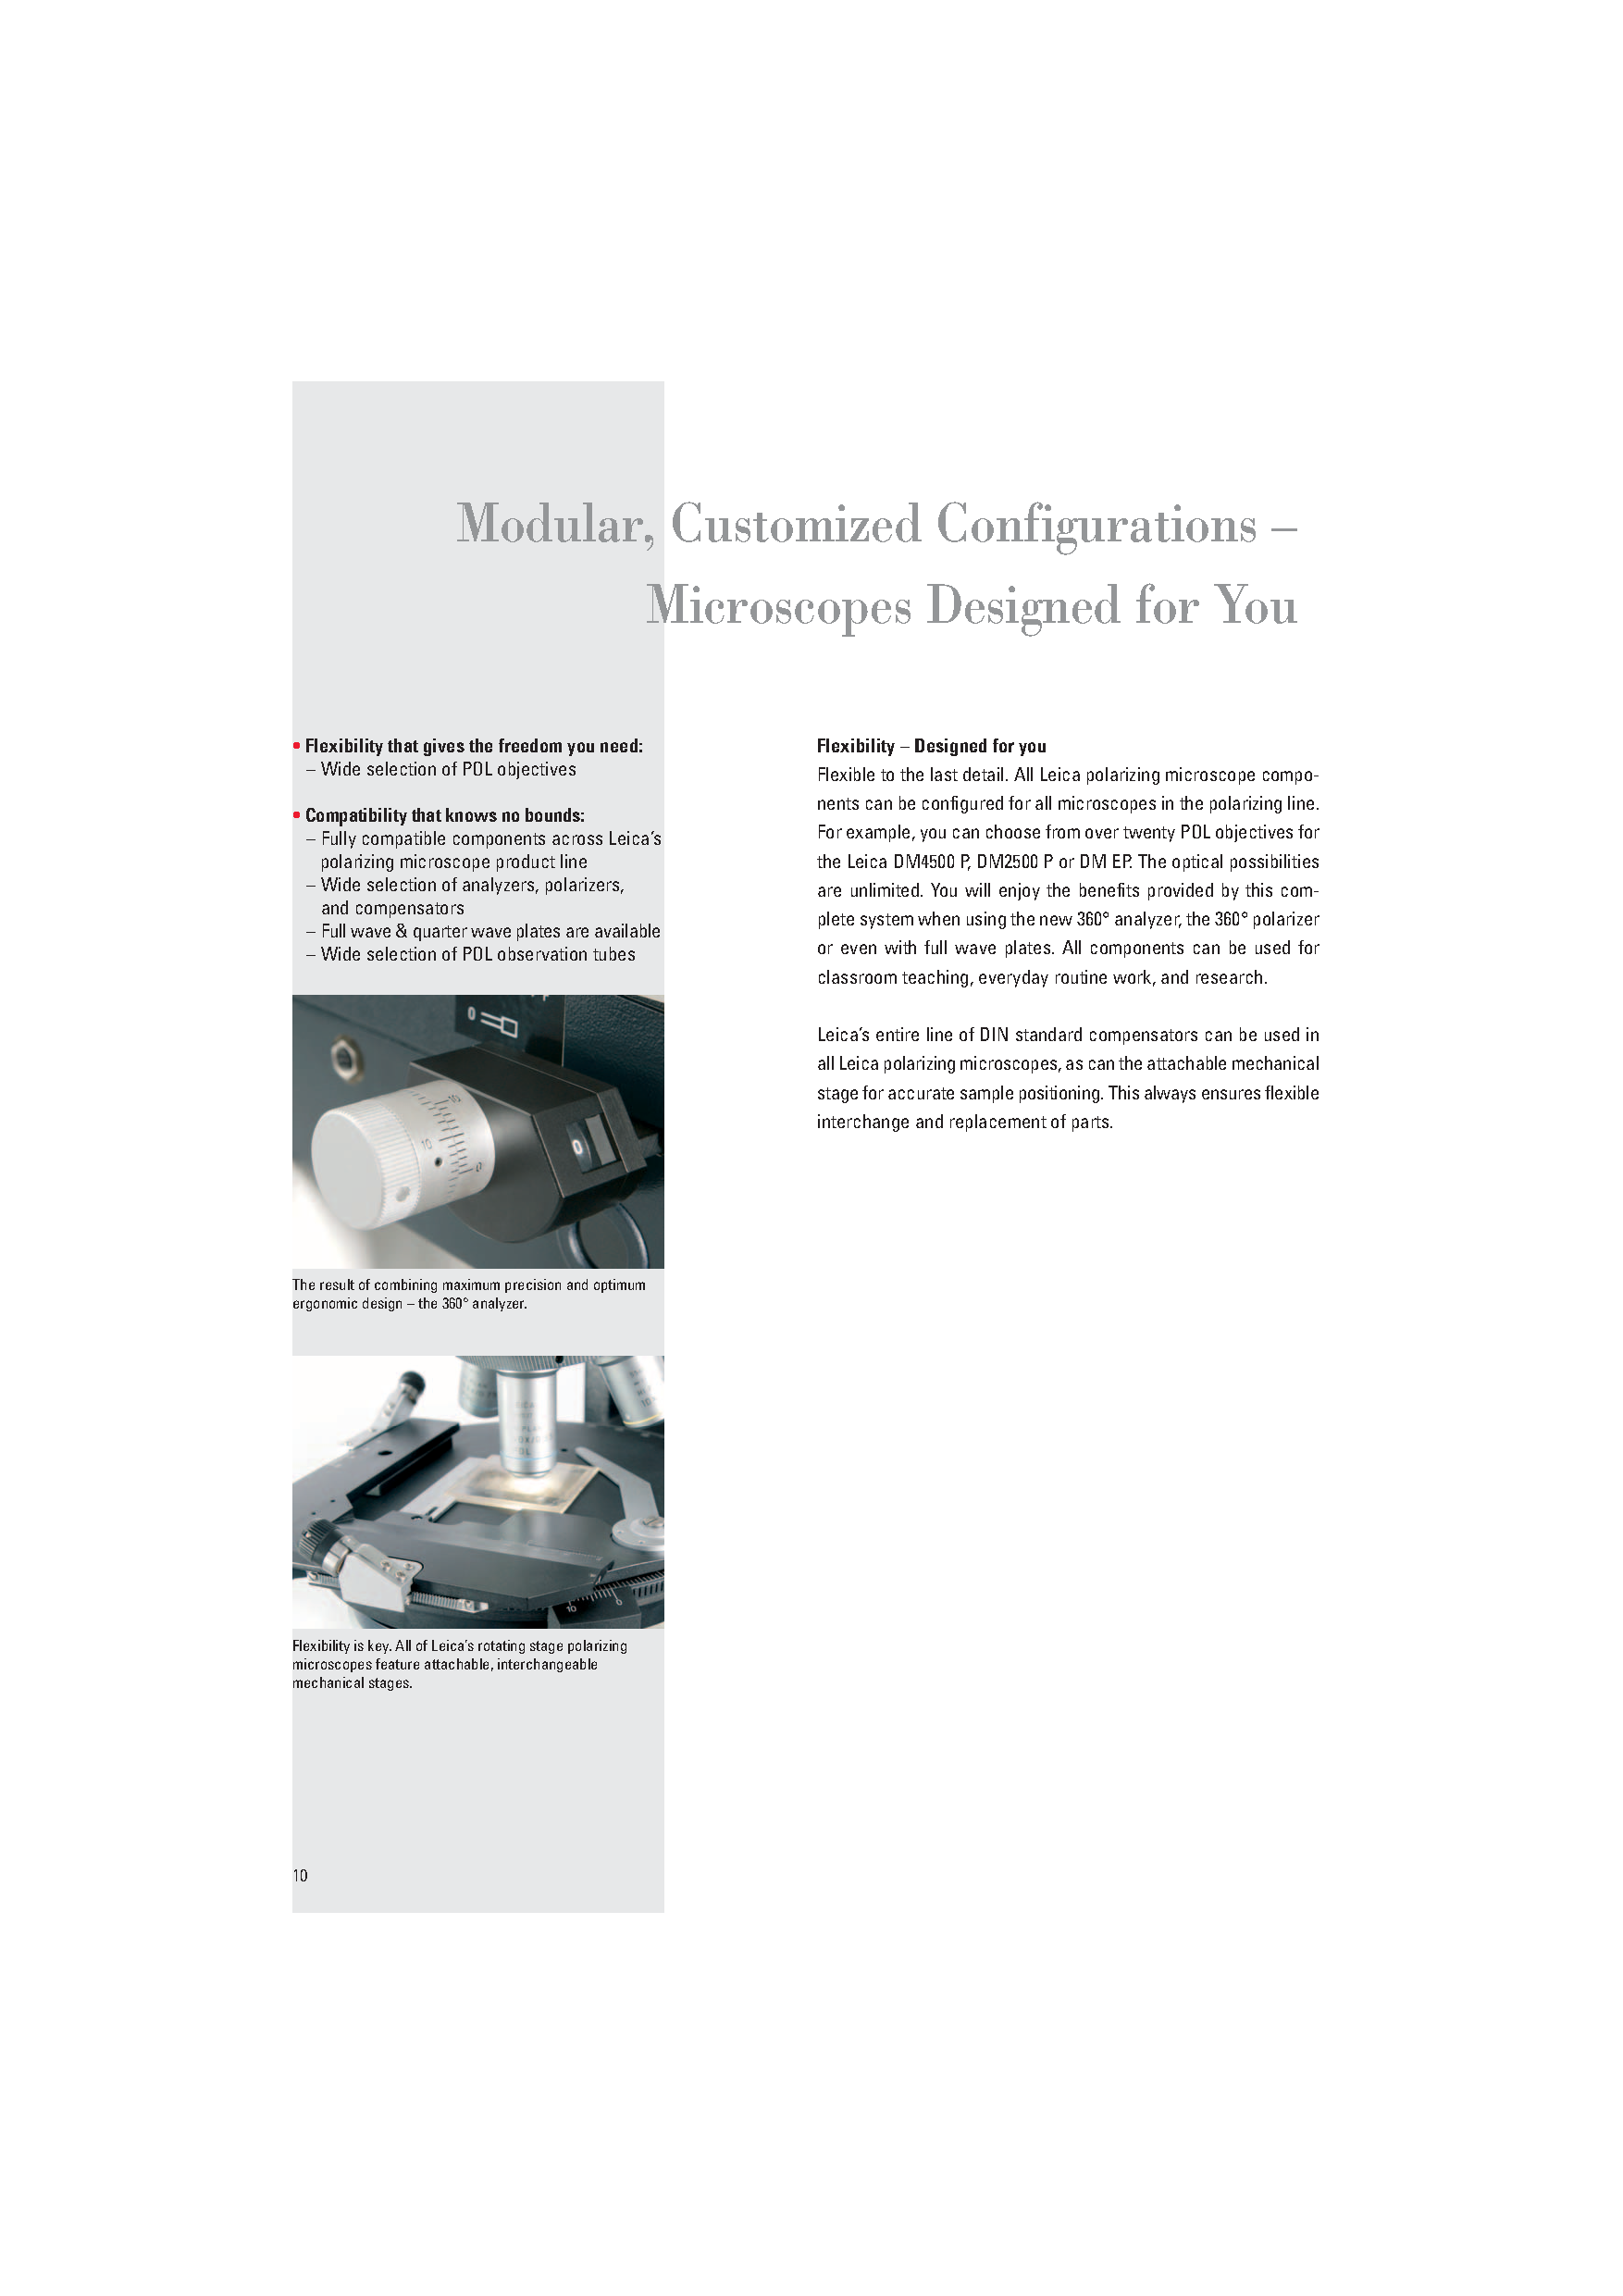
\includegraphics[width=0.9\textwidth]{afbeeldingen/manual_cut_3.pdf}
\end{figure}
\newpage
\begin{figure}[h!]
	\centering
	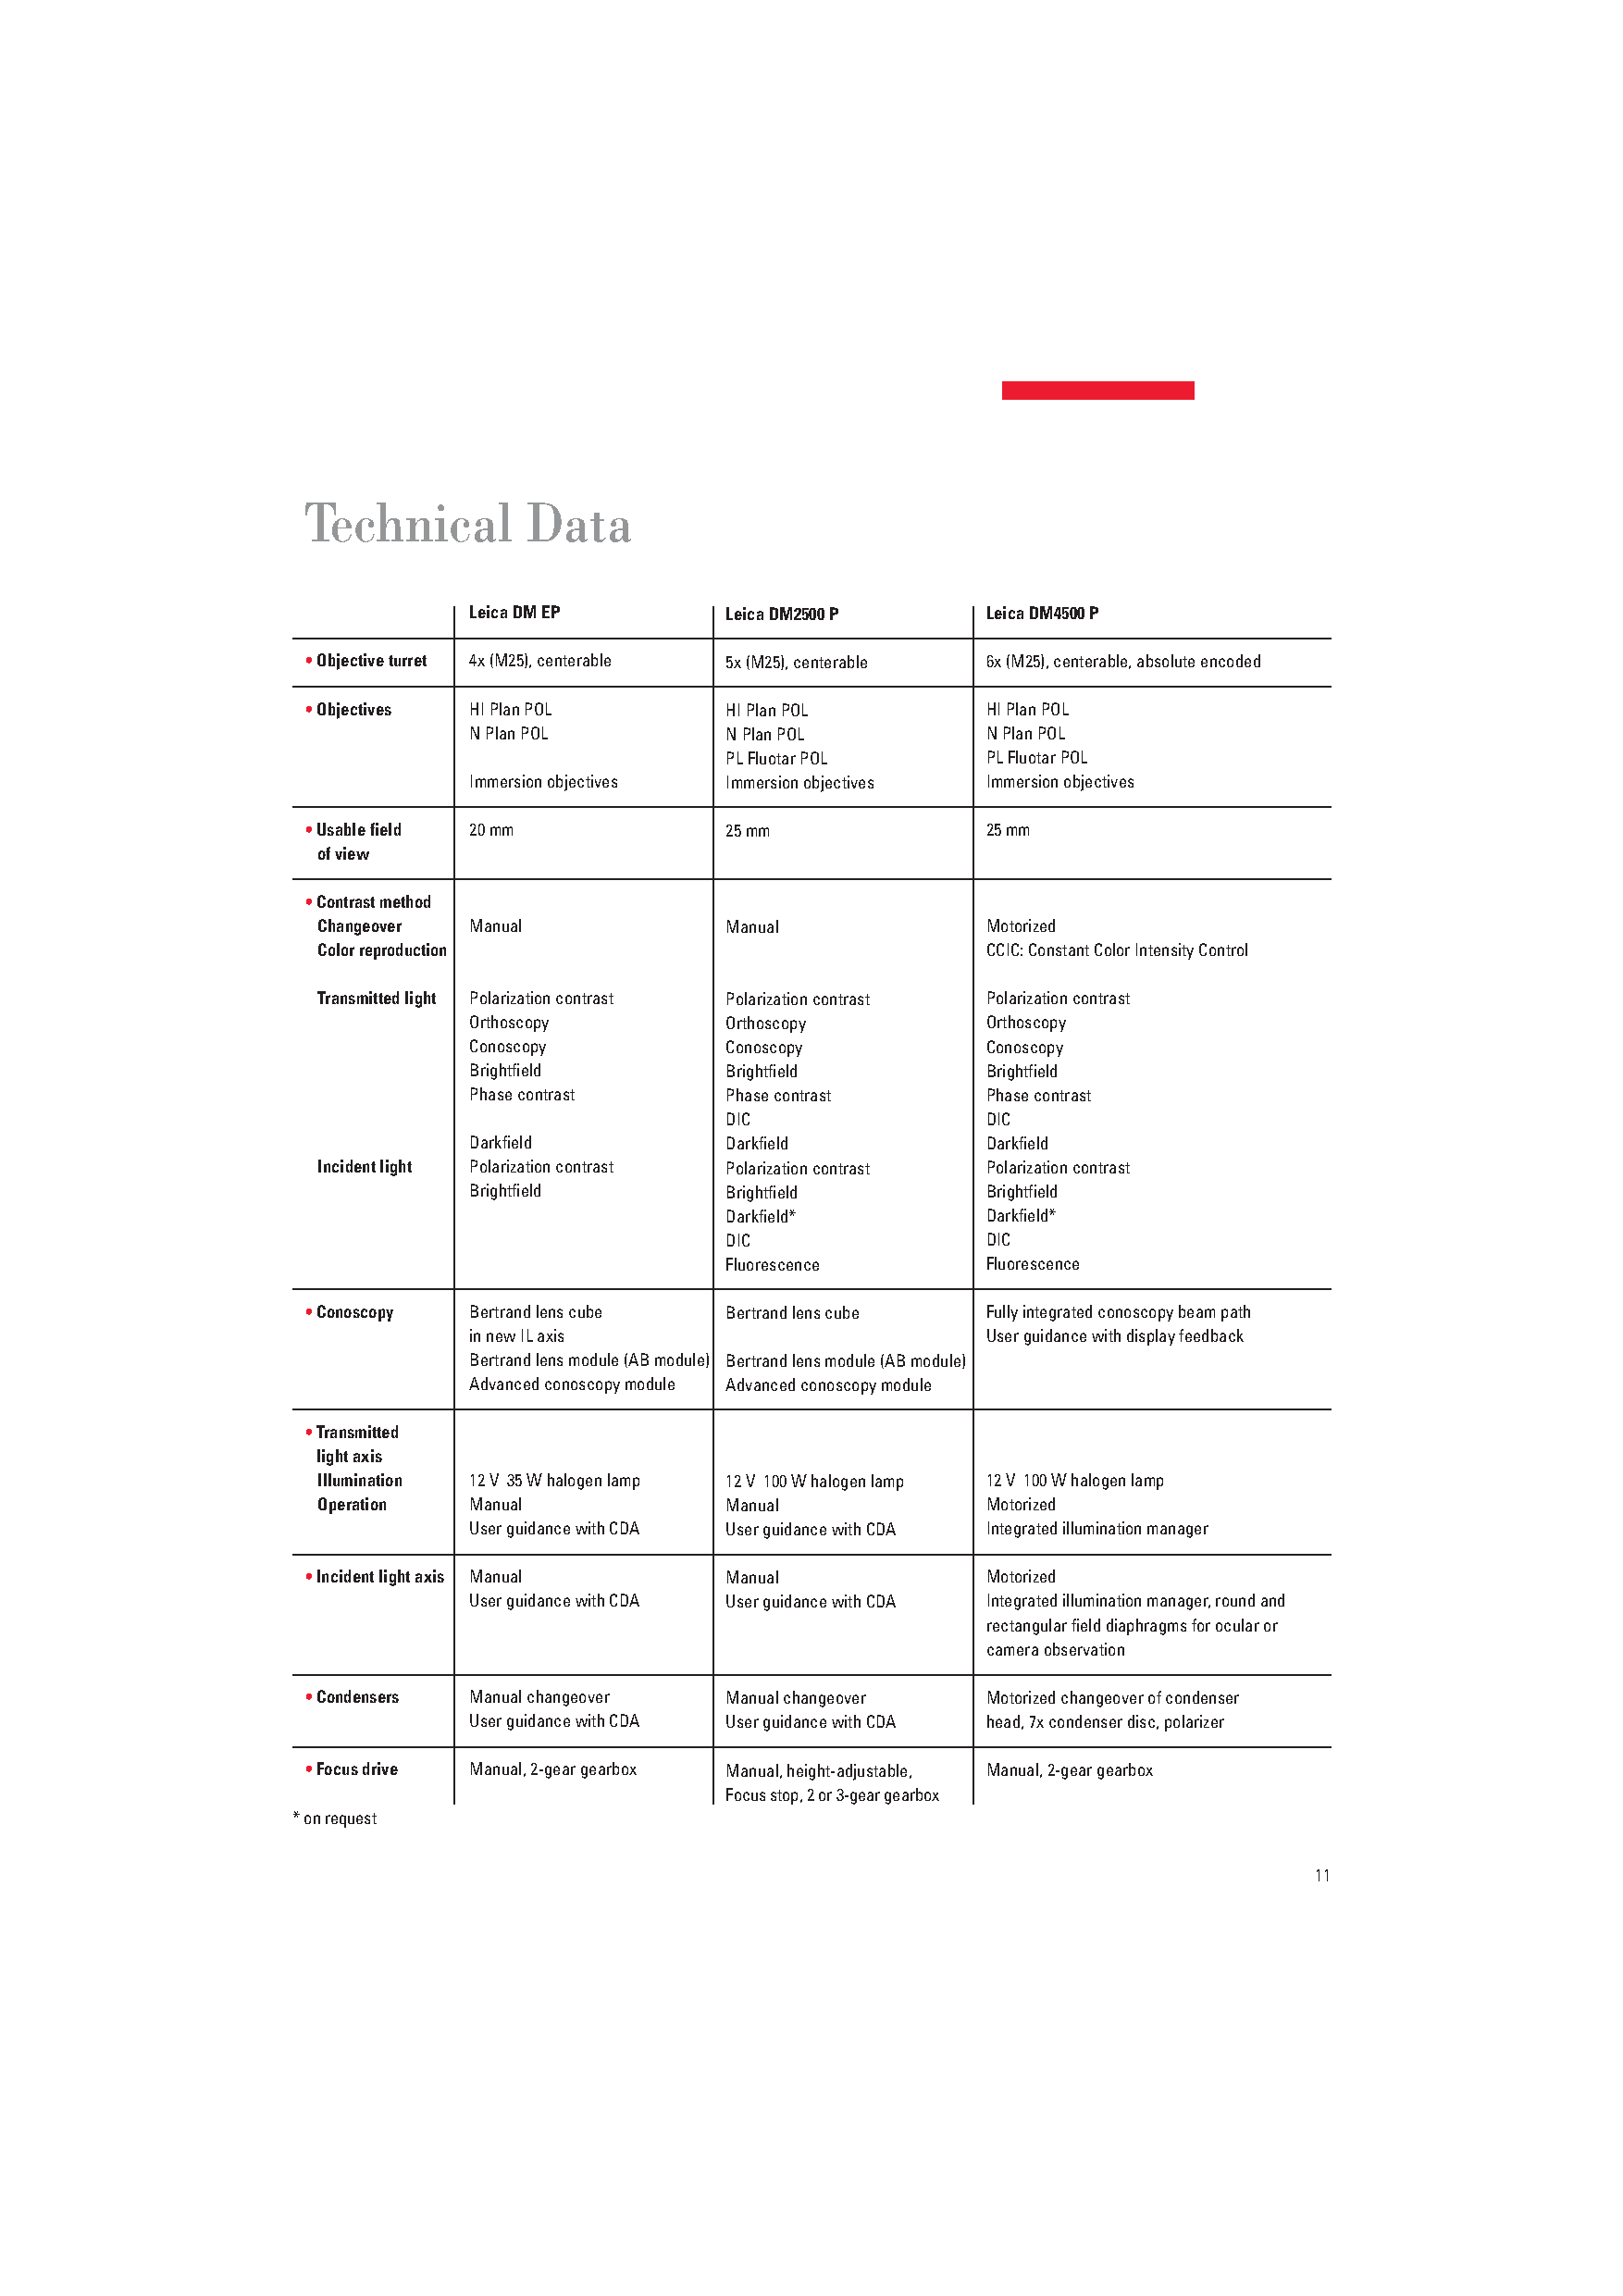
\includegraphics[width=0.9\textwidth]{afbeeldingen/manual_cut_2.pdf}
\end{figure}

\newpage
\subsection{Calibration}
\label{appendix_calibration}

The three images that are used to find $l_{pixel}$ for each objective can be found in figure \ref{fig_pixelszie_4x}, \ref{fig_pixelszie_10x} and \ref{fig_pixelszie_40x}.

\begin{figure}[h!]
    \centering
    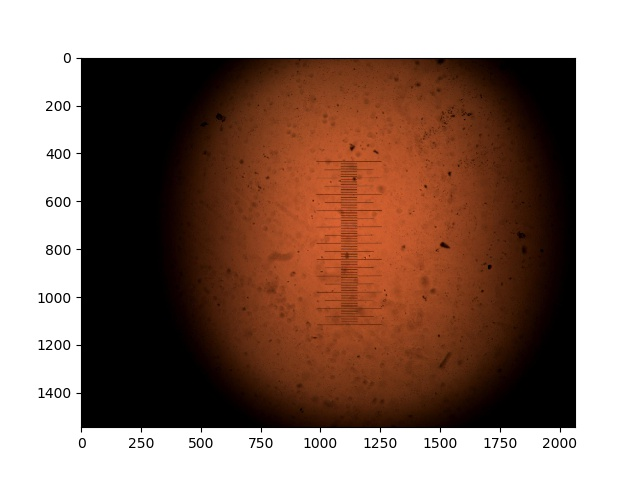
\includegraphics[width=7cm]{afbeeldingen/pixelsize/pixelsize_4x.jpg}
    \captionsetup{font=small, justification = centering}
    \caption{Image used to find $l_{pixel}$ for the $4\times$ objective.}
    \label{fig_pixelsize_4x}
\end{figure}

\begin{figure}[h!]
    \centering
    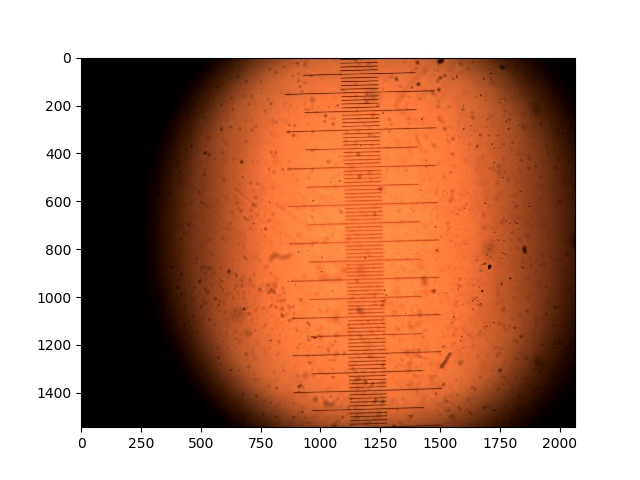
\includegraphics[width=7cm]{afbeeldingen/pixelsize/pixelsize_10x.jpg}
    \captionsetup{font=small, justification = centering}
    \caption{Image used to find $l_{pixel}$ for the $10\times$ objective.}
    \label{fig_pixelsize_10x}
\end{figure}

\begin{figure}[h!]
    \centering
    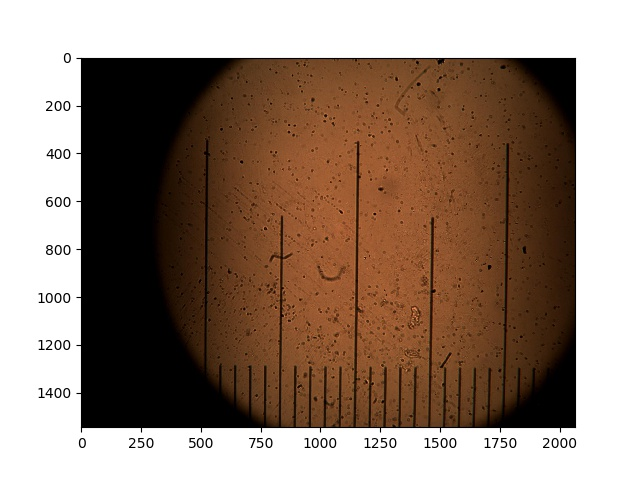
\includegraphics[width=7cm]{afbeeldingen/pixelsize/pixelsize_40x.jpg}
    \captionsetup{font=small, justification = centering}
    \caption{Image used to find $l_{pixel}$ for the $40\times$ objective.}
    \label{fig_pixelsize_40x}
\end{figure}
\newpage
\subsection{Size Measurements}
\label{appendix_size}

The images used to find $d_{hair}$ and $d_{gf}$ are presented in respectively figure \ref{fig_hair} and \ref{fig_gf}. The numbers on the axes correspond to the pixel count.

\begin{figure}[h!]
    \centering
    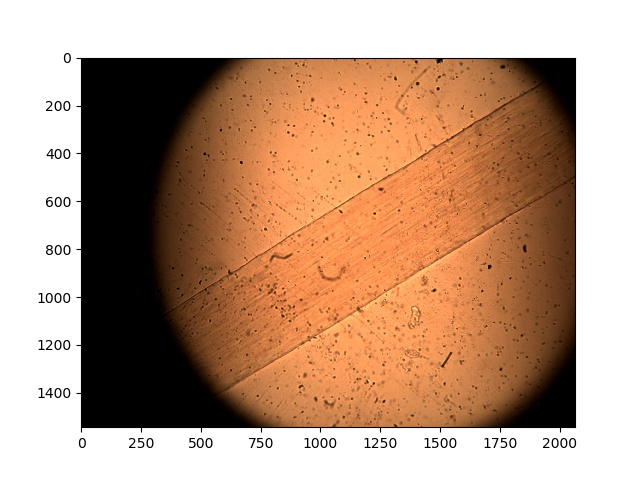
\includegraphics[width=7cm]{afbeeldingen/size/hair.jpg}
    \captionsetup{font=small, justification = centering}
    \caption{Image used to find $d_{hair}$.}
    \label{fig_hair}
\end{figure}

\begin{figure}[h!]
    \centering
    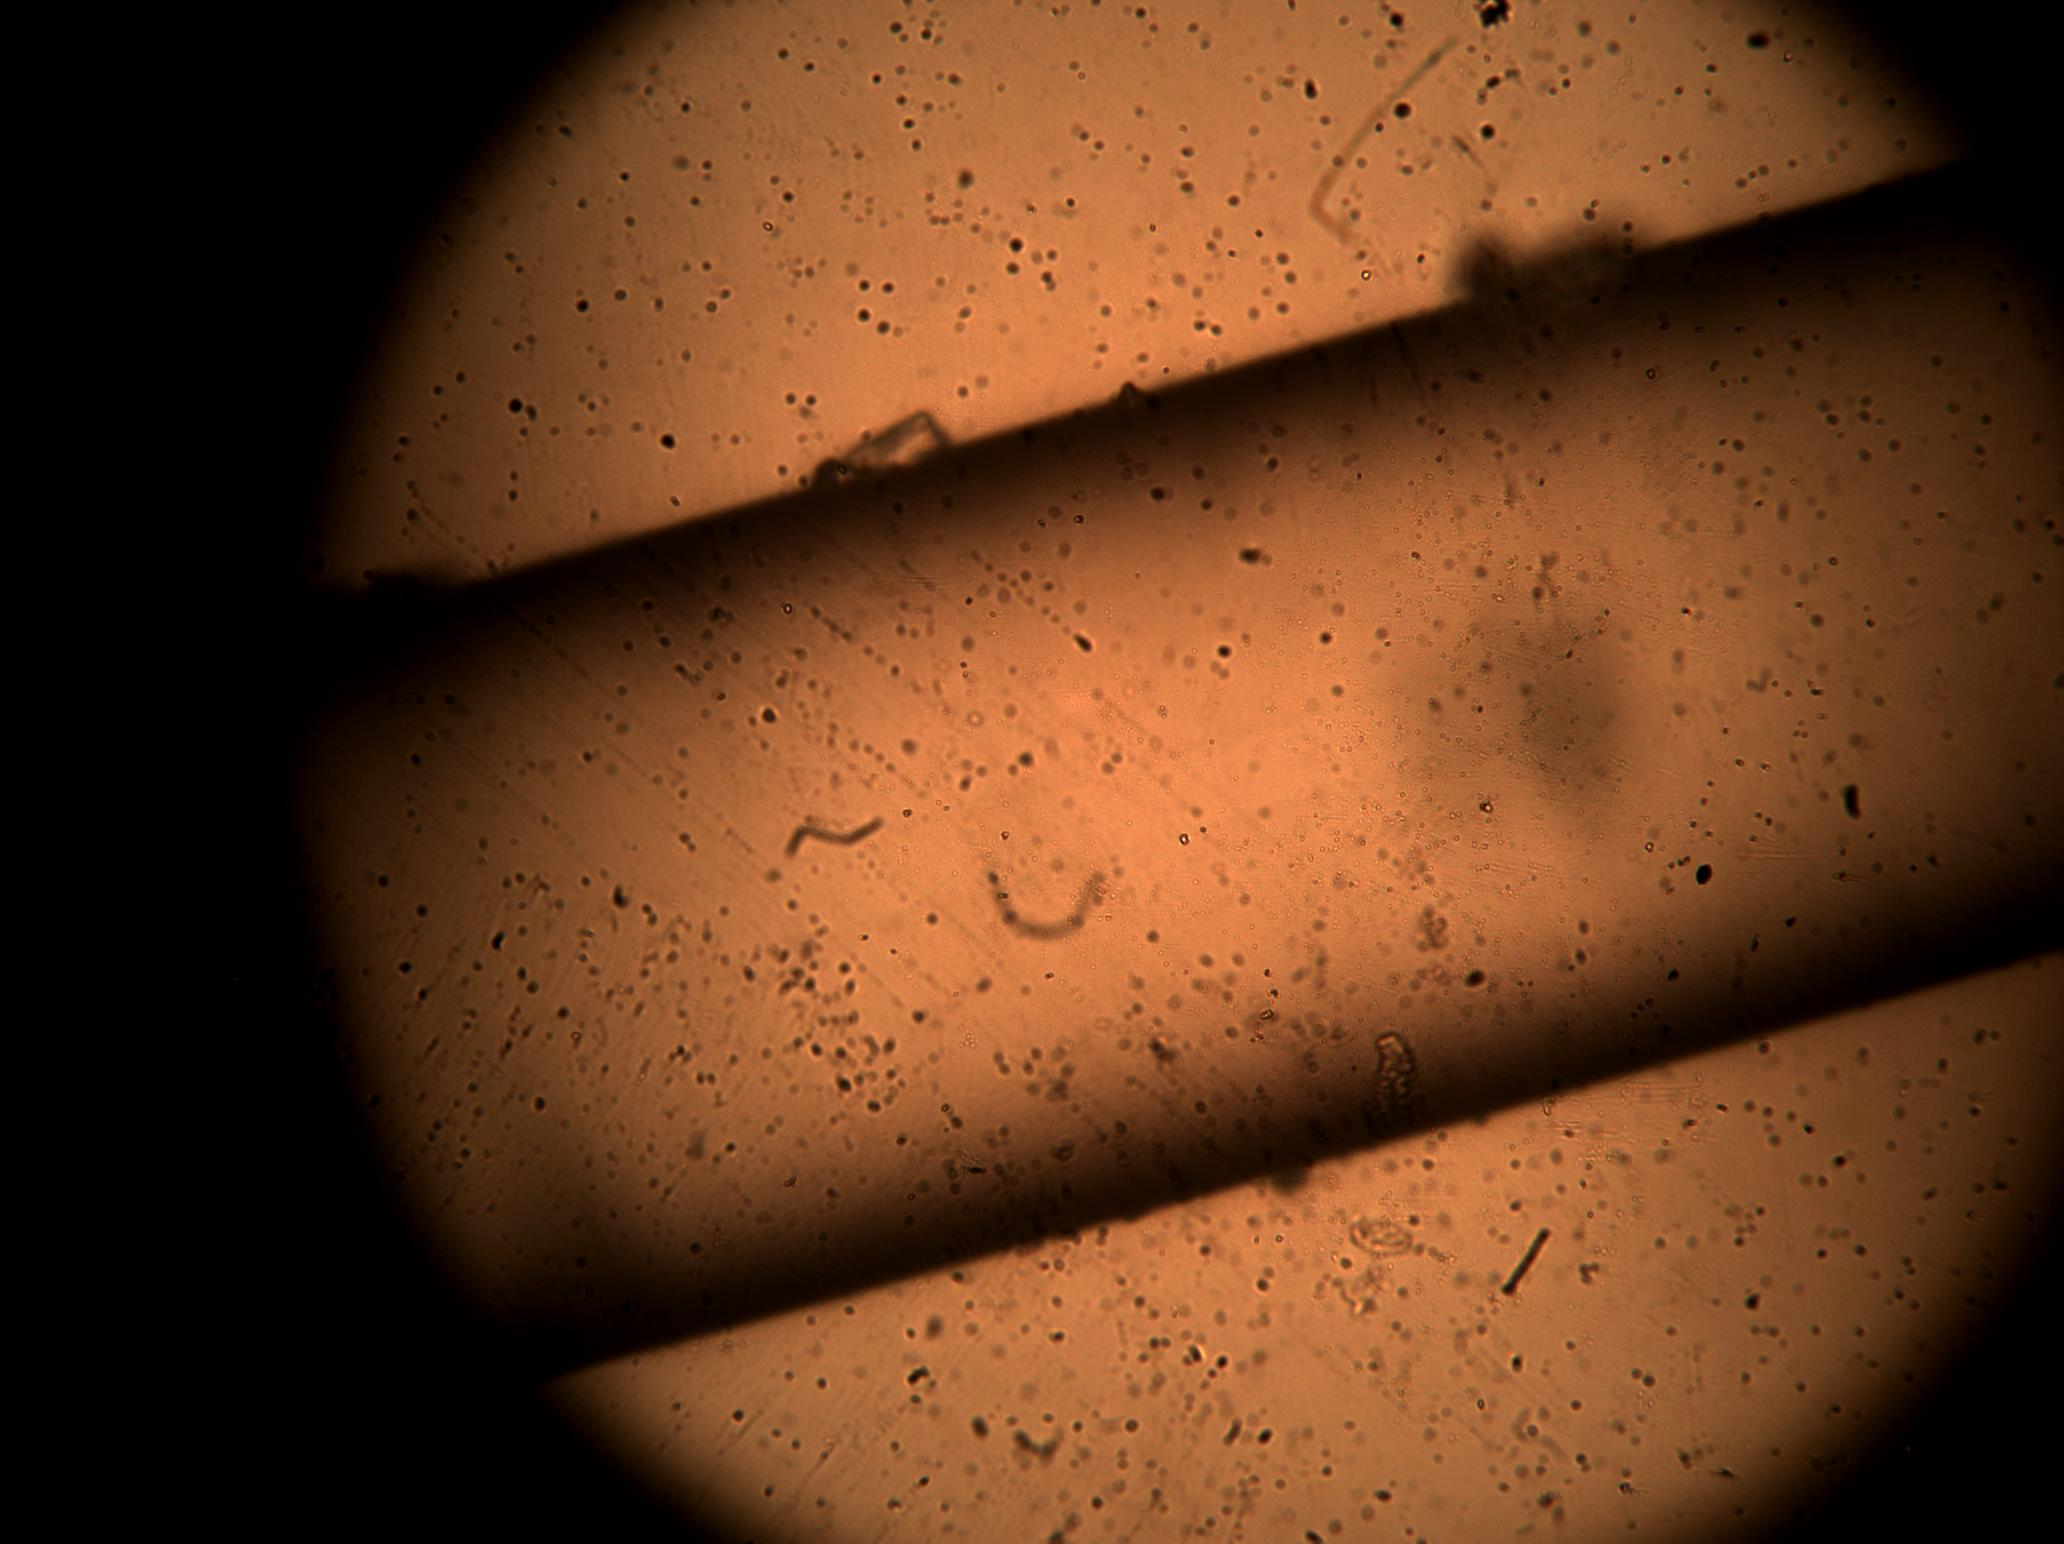
\includegraphics[width=7cm]{afbeeldingen/size/gf.jpg}
    \captionsetup{font=small, justification = centering}
    \caption{Image used to find $d_{gf}$.}
    \label{fig_gf}
\end{figure}

\newpage

The values that have been found for $a$, $b$, $A$ and the corresponding errors are presented in table \ref{table_zetmeel}.

\begin{table}[h!]
\centering
\captionsetup{font=small, justification = centering}
  \caption{Results of measurements of $a$ and $b$ for 30 starch particles. It was estimated that $u(a) =u(b) = 2 \: pixels$. The values for $A$ and $u(A)$ follow from equations \ref{eq_distance}, \ref{eq_u_distance}, \ref{eq_ellipse} and \ref{eq_u_ellipse}. The particles corresponding to each number can be seen in figures \ref{fig_zetmeel_1} to \ref{fig_zetmeel_6}.}

\begin{tabular}{|l|l|l|l|l|} \hline
Particle number & $a \: (\# pixels)$ & $b \:  (\# pixels)$ & $A \: \cdot 10^{-10} \; (m^2)$ & $u(A) \: \cdot 10^{-12} \; (m^2)$ \\ \hline
1               & 84                 & 76                 & 1.28                           & 5                                 \\
2               & 83                 & 75                 & 1.25                           & 5                                 \\
3               & 85                 & 77                 & 1.32                           & 5                                 \\
4               & 72                 & 67                 & 0.97                           & 4                                 \\
5               & 97                 & 94                 & 1.83                           & 6                                 \\
6               & 58                 & 58                 & 0.68                           & 3                                 \\
7               & 70                 & 66                 & 0.93                           & 4                                 \\
8               & 105                & 95                 & 2.01                           & 6                                 \\
9               & 92                 & 90                 & 1.67                           & 5                                 \\
10              & 84                 & 82                 & 1.39                           & 5                                 \\
11              & 115                & 115                & 2.66                           & 7                                 \\
12              & 146                & 128                & 3.76                           & 8                                 \\
13              & 119                & 110                & 2.63                           & 7                                 \\
14              & 76                 & 75                 & 1.15                           & 4                                 \\
15              & 112                & 108                & 2.43                           & 6                                 \\
16              & 127                & 125                & 3.19                           & 7                                 \\
17              & 99                 & 90                 & 1.79                           & 6                                 \\
18              & 84                 & 81                 & 1.37                           & 5                                 \\
19              & 135                & 123                & 3.34                           & 8                                 \\
20              & 80                 & 78                 & 1.26                           & 5                                 \\
21              & 86                 & 84                 & 1.45                           & 5                                 \\
22              & 112                & 106                & 2.39                           & 6                                 \\
23              & 105                & 103                & 2.18                           & 6                                 \\
24              & 74                 & 72                 & 1.07                           & 4                                 \\
25              & 117                & 116                & 2.73                           & 7                                 \\
26              & 90                 & 83                 & 1.50                           & 5                                 \\
27              & 100                & 91                 & 1.83                           & 6                                 \\
28              & 117                & 104                & 2.45                           & 6                                 \\
29              & 100                & 97                 & 1.95                           & 6                                 \\
30              & 99                 & 92                 & 1.83                           & 6\\ \hline
\end{tabular}
\label{table_zetmeel}
\end{table}

\newpage

The images that were used to find the data in table \ref{table_zetmeel} can been seen in figure \ref{fig_zetmeel}

\begin{figure}[h!]
	
    \begin{subfigure}[b]{0.475\textwidth}
        \centering
        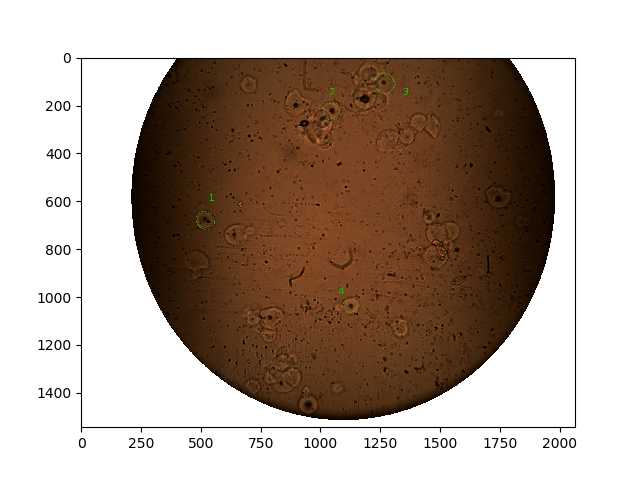
\includegraphics[width=\textwidth]{afbeeldingen/size/zetmeel/zetmeel_1.png}
        \caption{Best ellipse fits for starch particles 1 to 4.}   
        \label{fig_zetmeel_1}
    \end{subfigure}
    \hspace*{\fill}
    \begin{subfigure}[b]{0.475\textwidth}
        \centering
        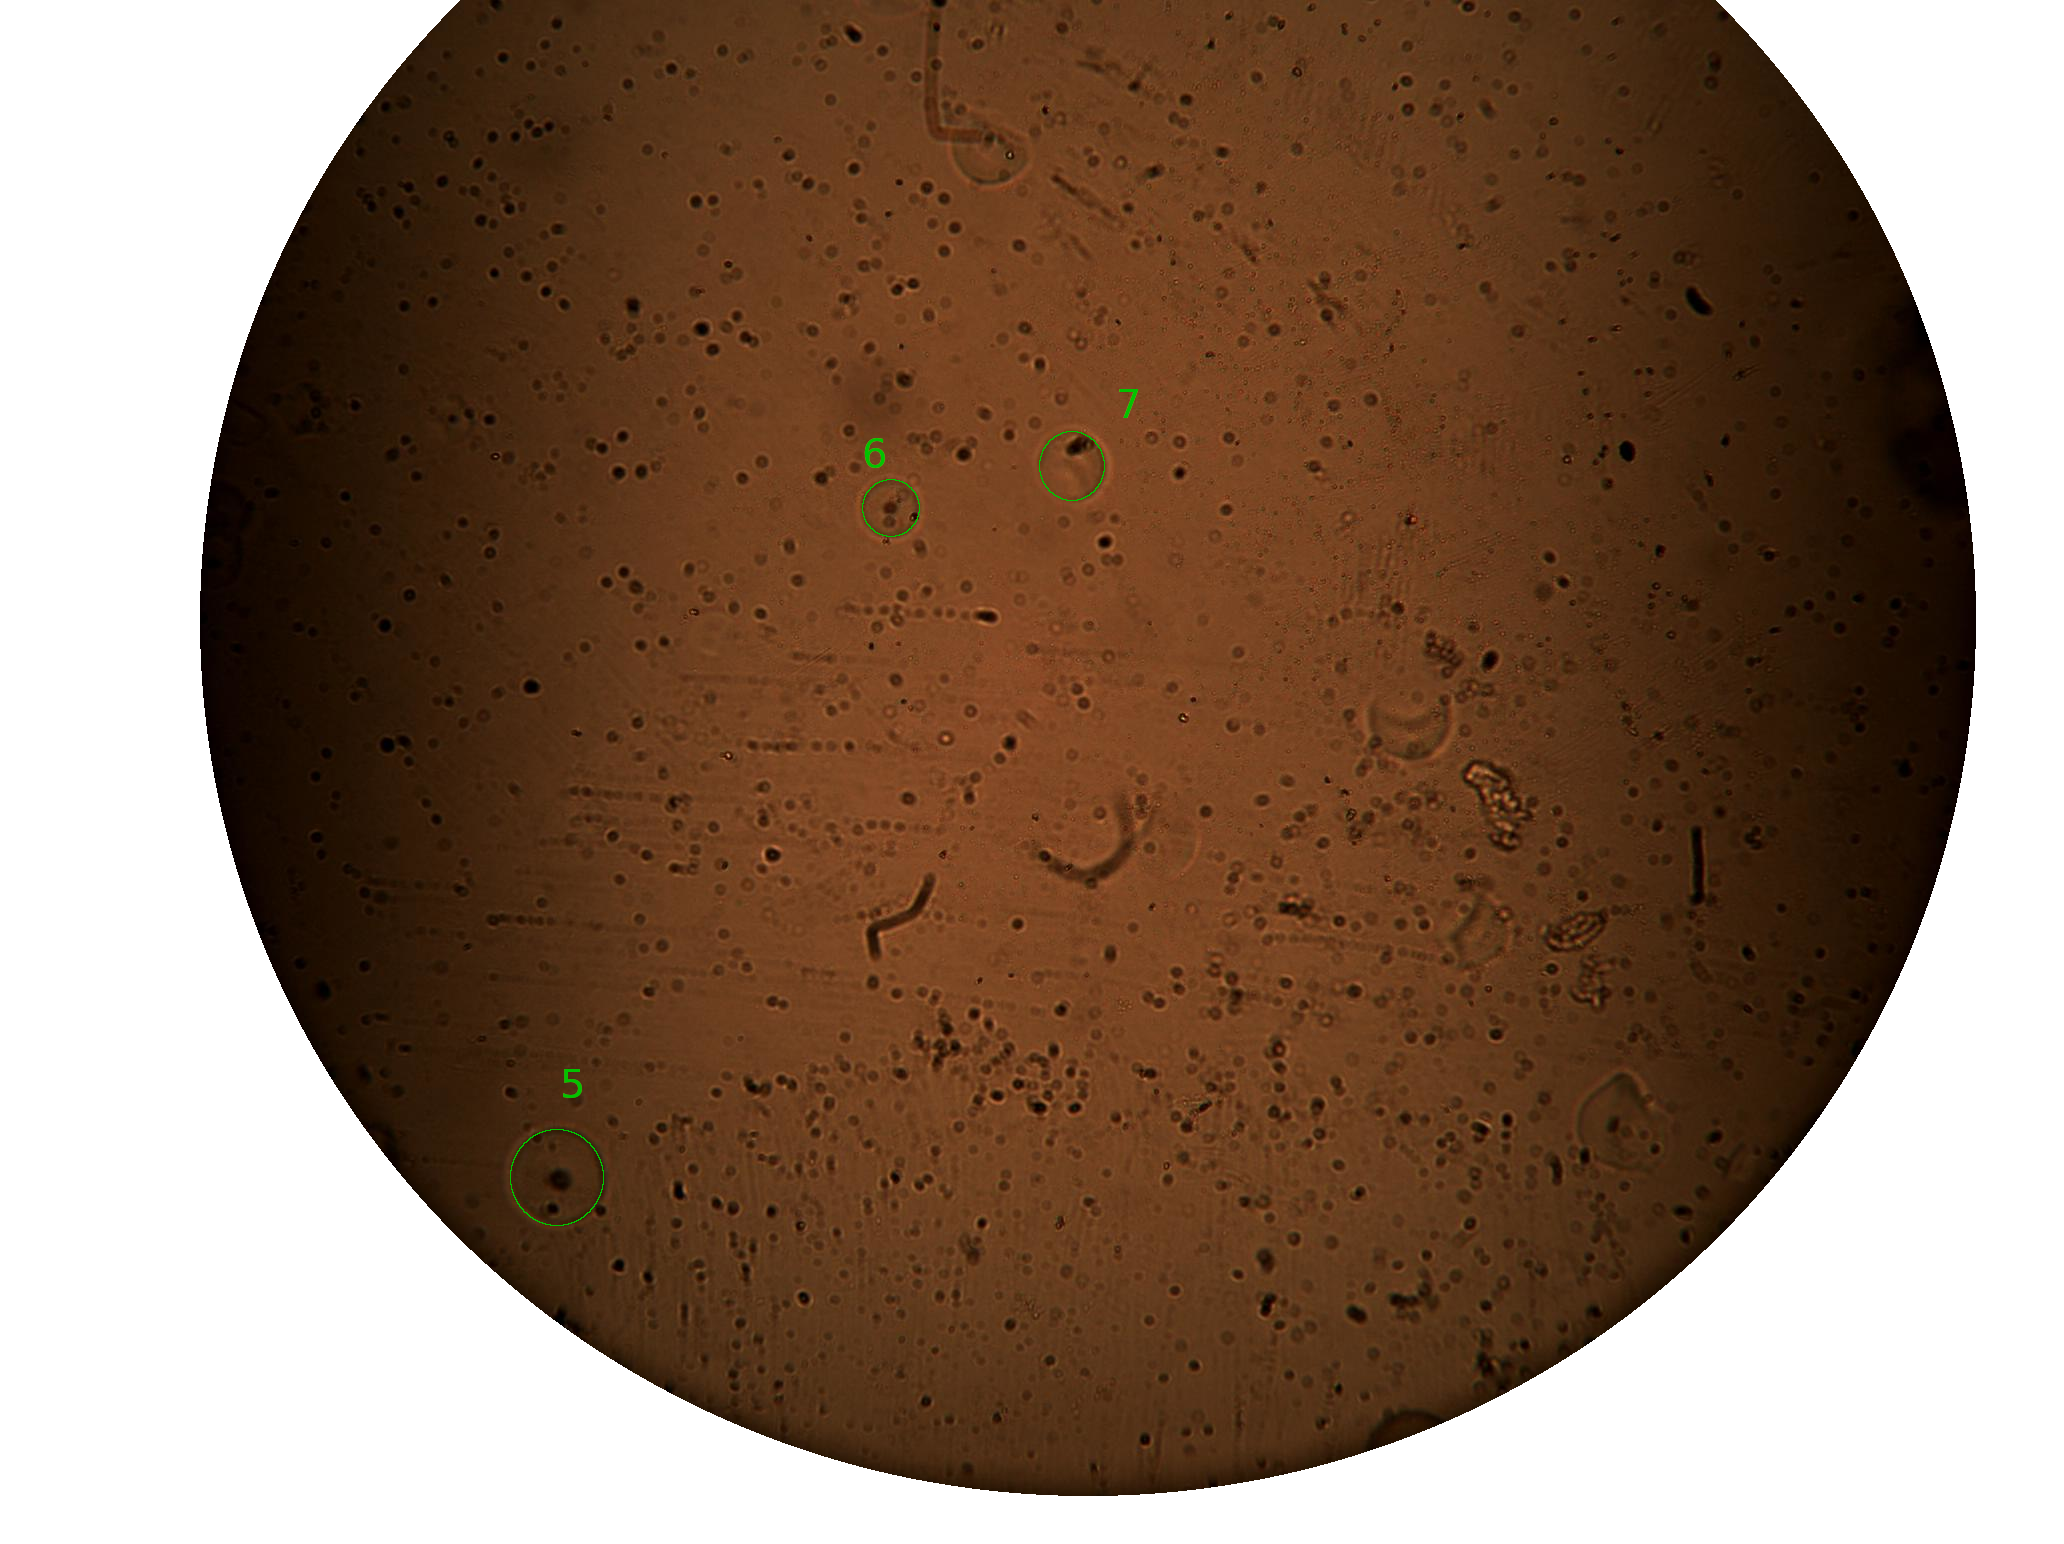
\includegraphics[width=\textwidth]{afbeeldingen/size/zetmeel/zetmeel_2.png}
        \caption{Best ellipse fits for starch particles 5 to 7.}   
        \label{fig_zetmeel_2}
    \end{subfigure}
    
    \medskip
    \begin{subfigure}[b]{0.475\textwidth}
        \centering
        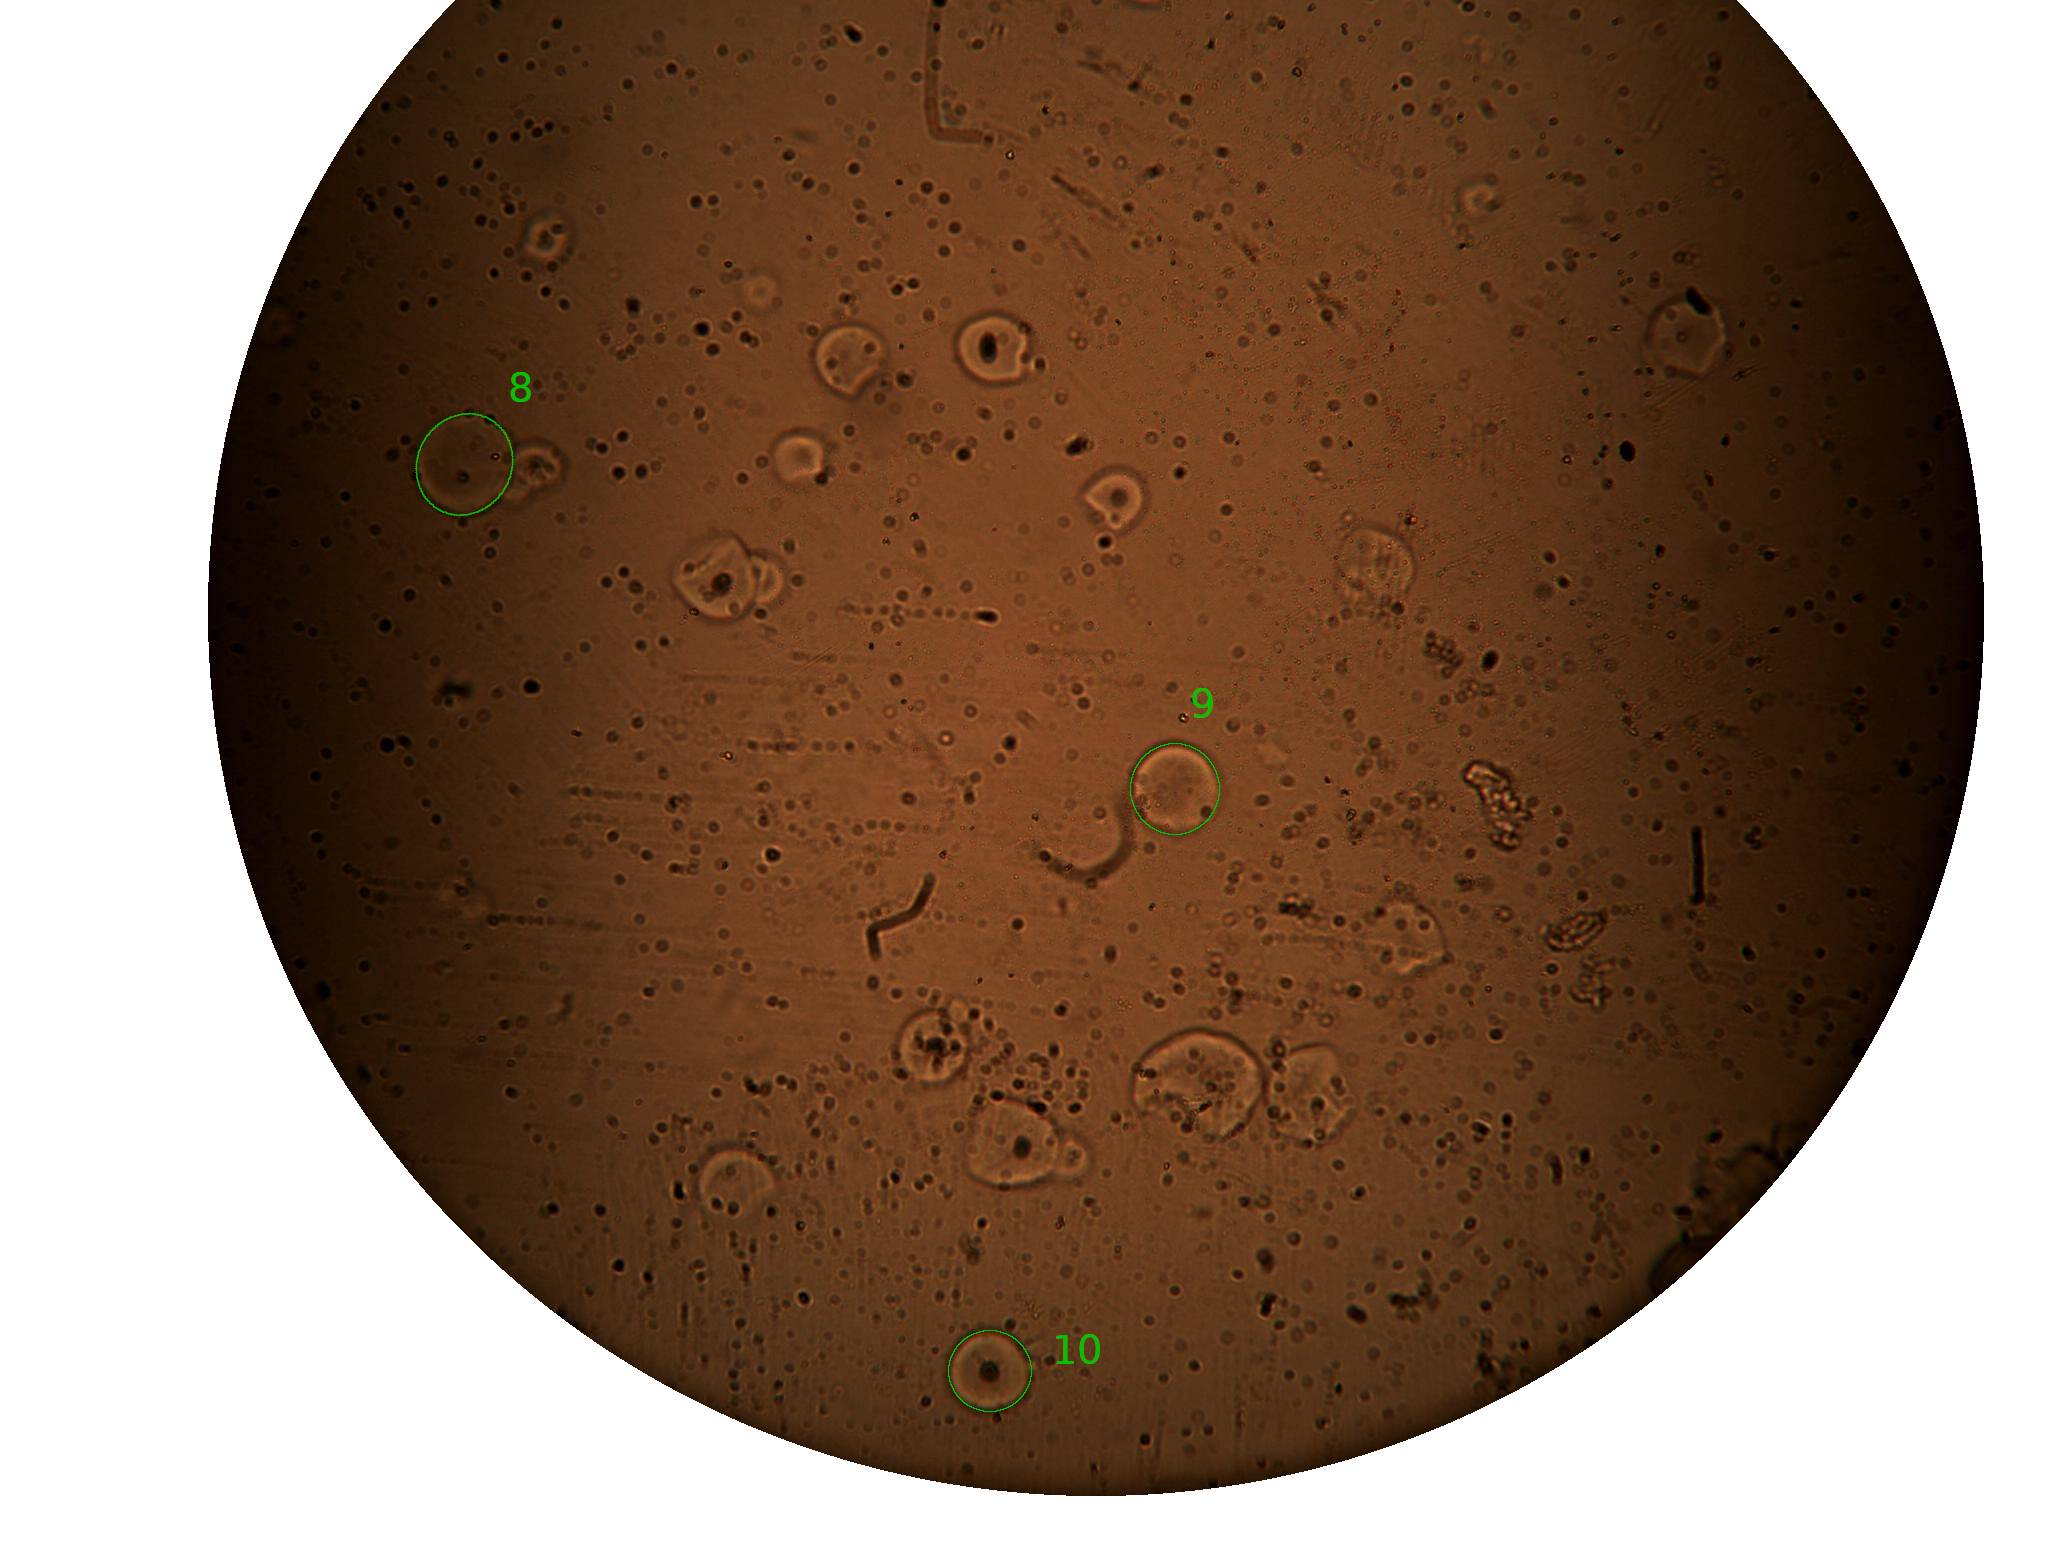
\includegraphics[width=\textwidth]{afbeeldingen/size/zetmeel/zetmeel_3.png}
        \caption{Best ellipse fits for starch particles 8 to 10.}   
        \label{fig_zetmeel_3}
    \end{subfigure}
    \hspace*{\fill}
    \begin{subfigure}[b]{0.475\textwidth}
        \centering
        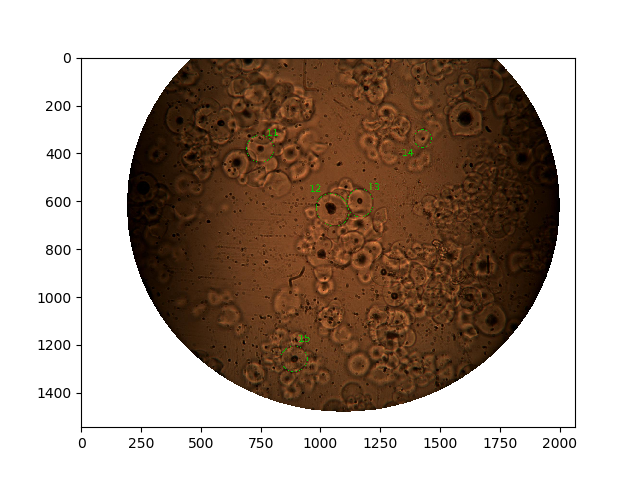
\includegraphics[width=\textwidth]{afbeeldingen/size/zetmeel/zetmeel_4.png}
        \caption{Best ellipse fits for starch particles 11 to 15.}   
        \label{fig_zetmeel_4}
    \end{subfigure}
    
    \medskip
    \begin{subfigure}[b]{0.475\textwidth}
        \centering
        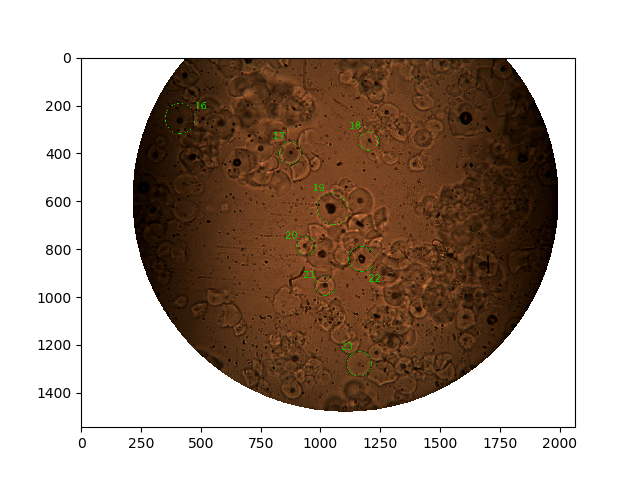
\includegraphics[width=\textwidth]{afbeeldingen/size/zetmeel/zetmeel_5.png}
        \caption{Best ellipse fits for starch particles 16 to 23.}   
        \label{fig_zetmeel_5}
    \end{subfigure}
    \hspace*{\fill}
    \begin{subfigure}[b]{0.475\textwidth}
        \centering
        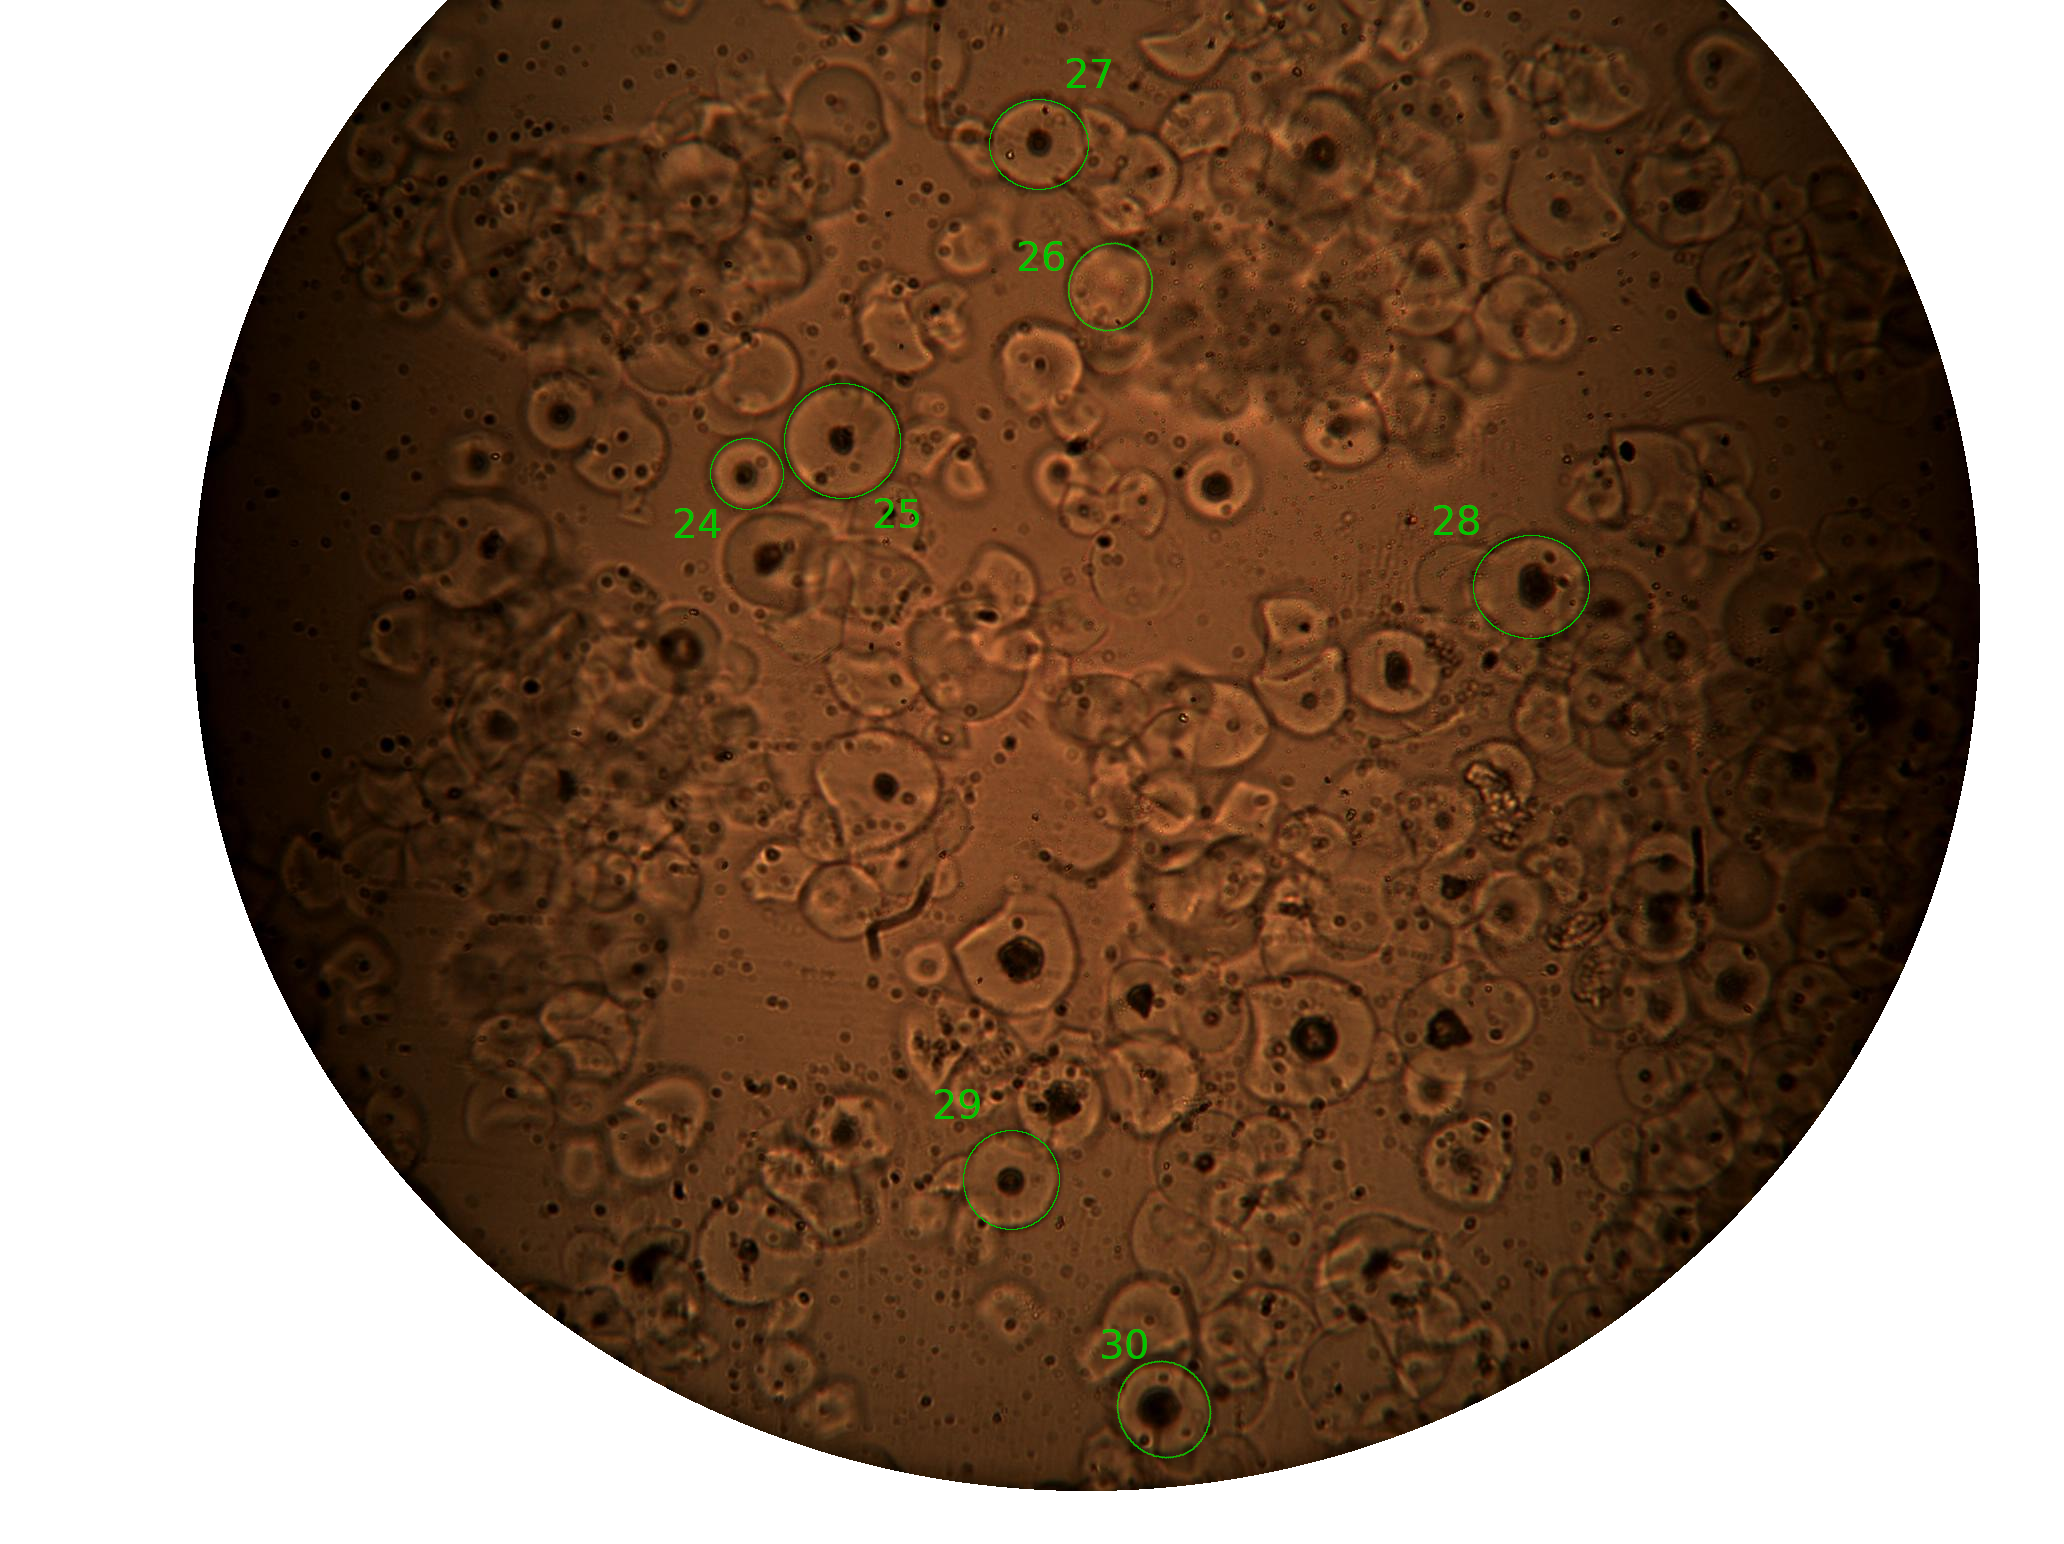
\includegraphics[width=\textwidth]{afbeeldingen/size/zetmeel/zetmeel_6.png}
        \caption{Best ellipse fits for starch particles 24 to 30.}   
        \label{fig_zetmeel_6}
    \end{subfigure}
    
    \caption{Set of images used to find best ellipse fits for 30 starch particles. The green ellipses represent the best fit. The numbers on the axes, correspond to the pixel count.} 
	\label{fig_zetmeel}
\end{figure}

\newpage
\subsection{Birefringence}
\label{appendix_bf}

The results for $f$ for each colour plane is presented in table \ref{table_bf_f}. It was estimated that $u(f) = 2 \cdot 10^{-6} \: (m)$. 

\begin{table}[h!]
\captionsetup{font=small, justification = centering}
  \caption{Results of measurements of $f$. The Roman numerals represent the different colour planes (see figure \ref{fig_bf_planes}). The letters A, B, C and D represent different measurements at different locations of the sample.}
\begin{adjustbox}{width=1\textwidth}
\begin{tabular}{|l|l|l|l|l|l|l|l|l|} \hline
\multicolumn{2}{|l|}{A}                                          & \multicolumn{3}{l|}{B}                                                                & \multicolumn{2}{l|}{C}                                   & \multicolumn{2}{l|}{D}                                   \\ \hline
$f_{bottom} \cdot 10^{-5} \: (m)$ & $f_{II} \cdot 10^{-5} \: (m)$ & $f_{II} \cdot 10^{-5} \: (m)$ & $f_{III} \cdot 10^{-5} \: (m)$ & $f_{V} \cdot 10^{-5} \: (m)$ & $f_{III} \cdot 10^{-5} \: (m)$ & $f_{IV} \cdot 10^{-5} \: (m)$ & $f_{I} \cdot 10^{-5} \: (m)$ & $f_{II} \cdot 10^{-5} \: (m)$ \\ \hline
1.5                               & 2.5                        & 2.2                        & 2.4                        & 3.3                        & 7.0                        & 6.5                        & 6.0                        & 6.4                        \\
1.4                               & 2.5                        & 2.3                        & 2.4                        & 3.5                        & 7.1                        & 6.5                        & 6.0                        & 6.5                        \\
1.5                               & 2.5                        & 2.3                        & 2.5                        & 3.7                        & 7.0                        & 6.5                        & 6.1                        & 6.5                        \\
1.6                               & 2.5                        & 2.4                        & 2.6                        & 3.7                        & 3.0                        & 6.5                        & 6.1                        & 6.4                        \\
                                  &                            & 2.6                        & 2.8                        & 3.4                        & 7.1                        & 6.6                        & 6.0                        & 6.5                       \\ \hline
\end{tabular}
\end{adjustbox}
\label{table_bf_f}
\end{table}

The values for $D$ follow from the values of $f$. The values for $D$, $\Delta l_{path}$ and the corresponding errors are presented in table \ref{table_bf}.

\begin{table}[h!]
	\caption{Results for measurements of $D$, $\Delta l_{path}$ and the corresponding errors for each colour plane (see figure \ref{fig_bf_planes}). The values of $D$ were found with simple addition and subtraction using the values of $f$. The values of $\Delta l_{path}$ were found using a Michel-L\'evy birefringence chart (\cite{bf_chart}).}
\begin{tabular}{|l|l|l|l|l|} \hline
Colour Plane & $D  \: \cdot 10^{-5}  \: (m)$ & $u(D) \:  \cdot 10^{-6} \: (m) $ & $\Delta l_{path} \:  \cdot 10^{-7} \: (m) $ & $u(\Delta l_{path})  \:  \cdot 10^{-8} \: (m)$ \\ \hline
I            & 0.6                           & 2                                & 2.7                                         & 2                                              \\
II           & 1.0                           & 1                                & 5.1                                         & 1                                              \\
III          & 1.2                           & 2                                & 6.0                                         & 1                                              \\
IV           & 1.7                           & 2                                & 11.9                                        & 2                                              \\
V            & 2.2                           & 2                                & 12.1                                        & 2                 \\ \hline
\end{tabular}
\label{table_bf}
\end{table}






\end{appendix}

\end{document}